\documentclass[12pt,a4paper]{article}
\usepackage[a4paper,top=1in,bottom=1in,left=1in,right=1in]{geometry}
\usepackage{graphicx}
\usepackage{xcolor}
\usepackage{setspace}
\usepackage{booktabs}
\usepackage{array}
\usepackage{amsmath}
\PassOptionsToPackage{hyphens}{url}
\usepackage{hyperref}
\usepackage{listings}
\usepackage{caption}
\usepackage{float}
\usepackage{enumitem}
\usepackage{parskip}
\usepackage{tikz}
\usetikzlibrary{shapes.geometric, arrows.meta, positioning}

\hypersetup{
    colorlinks=true,
    linkcolor=teal,
    urlcolor=blue!70!black,
    citecolor=teal
}

\lstset{
    language=Python,
    basicstyle=\ttfamily\small,
    keywordstyle=\color{blue!70!black}\bfseries,
    commentstyle=\color{gray},
    stringstyle=\color{red!60!black},
    backgroundcolor=\color{gray!8},
    frame=single,
    rulecolor=\color{gray!40},
    breaklines=true,
    showstringspaces=false,
    numbers=left,
    numberstyle=\tiny\color{gray},
    numbersep=6pt,
    xleftmargin=15pt
}

\begin{document}

% ---------------- COVER PAGE ----------------
\begin{center}

% -------- LOGO --------

\includegraphics[width=4.5cm]{LOGO.pdf}\\[0.5cm]

% -------- UNIVERSITY NAME --------
{\Large \textbf{SIKSHA 'O' ANUSANDHAN}}\\
{\small (Deemed To Be University)}\\
{\small \textcolor{blue!60!black}{Accredited (3rd Cycle) by NAAC with A++ Grade}}\\[0.5cm]

\textcolor{gray}{\rule{12cm}{0.4pt}}\\[0.5cm]

Admission Batch: \textbf{2023} \hspace{1cm} Session: \textbf{2025--26}\\[1cm]

% -------- TITLE BLOCK --------
{\Large \textbf{\textcolor{teal}{Major Project Report}}}\\[0.3cm]

{\large \textbf{of}}\\[0.3cm]

{\large \textbf{\textcolor{purple}{MACHINE LEARNING CONCEPT -2 (CSE 3968)}}}\\[0.8cm]

{\large \textbf{On}}\\[0.3cm]

{\Huge \textbf{\textcolor{red!70!black}{Disease Prediction System\\[0.2cm]Using Machine Learning}}}\\[1cm]

% -------- STUDENTS --------
\textbf{\large Submitted by:}\\[0.5cm]

\begin{tabular}{ll}
1) NAME 1 & 2341\_\_\_\_\_ \\
2) NAME 2 & 2341\_\_\_\_\_ \\
3) NAME 3 & 2341\_\_\_\_\_ \\
4) NAME 4 & 2341\_\_\_\_\_ \\
\end{tabular}

\vspace{1cm}

Section: \textbf{2341\_\_\_} \hspace{0.8cm}
Semester: \textbf{\_\_\_\_\_\_} \hspace{0.8cm}
Branch: \textbf{\_\_\_\_\_\_}

\vspace{1.2cm}

% -------- FOOTER --------
{\small
Department of Computer Science \& Engineering\\
\textbf{Institute of Technical Education and Research (ITER), Siksha `O' Anusandhan Deemed to be University}\\
Jagamohan Nagar, Jagamara, Bhubaneswar, Odisha -- 751030
}

\vfill

\textbf{(May, 2026)}

\end{center}

\newpage

% ---------------- DECLARATION ----------------
\newpage
\begin{center}

{\Large \textbf{DECLARATION}}\\[1cm]

\end{center}

\noindent
We hereby declare that the project report entitled

\begin{center}
\textbf{``Disease Prediction System Using Machine Learning''}
\end{center}

\noindent
is a bonafide record of the work carried out by us during the 6\textsuperscript{th} semester of the Bachelor of Technology program in Computer Science and Engineering for the course \textbf{Machine Learning Concept - 2 (CSE 3968)}, under the regulations of Siksha `O' Anusandhan Deemed to be University.

\vspace{0.5cm}

\noindent
This work has been carried out under the guidance of the project supervisor and has not been submitted elsewhere for any academic evaluation or certification. We further declare that there are \textbf{no competing interests} associated with this project.

\vspace{1cm}

\noindent
\textbf{Submitted by:}

\vspace{0.5cm}

\begin{tabular}{p{6cm} p{6cm}}
NAME 1 (Regd. No: 2341\_\_\_\_\_) & Signature: \rule{5cm}{0.4pt} \\
\\
NAME 2 (Regd. No: 2341\_\_\_\_\_) & Signature: \rule{5cm}{0.4pt} \\
\\
NAME 3 (Regd. No: 2341\_\_\_\_\_) & Signature: \rule{5cm}{0.4pt} \\
\\
NAME 4 (Regd. No: 2341\_\_\_\_\_) & Signature: \rule{5cm}{0.4pt} \\
\end{tabular}

\vspace{1.5cm}

\noindent
\textbf{Project Supervisor:} \\
\vspace{0.5cm}
Name: \rule{8cm}{0.4pt} \\
\vspace{0.3cm}
Signature: \rule{6cm}{0.4pt}

\vfill

\begin{center}
Department of Computer Science \& Engineering\\
Institute of Technical Education and Research (ITER)\\
Siksha `O' Anusandhan Deemed to be University\\
Bhubaneswar, Odisha\\[0.5cm]

\textbf{Date:} \rule{4cm}{0.4pt}
\end{center}

\newpage

% ---------------- TOC ----------------
\tableofcontents
\newpage

% ================================================================
\section{Abstract}
% ================================================================

Getting a proper diagnosis at the right time can genuinely be the difference between a smooth recovery and something far more serious. The frustrating reality, especially in smaller towns and rural pockets of India, is that most people simply do not have dependable access to a doctor each time they fall ill. This project was put together with that problem squarely in mind. We developed a \textbf{Disease Prediction System} that accepts a patient's age and self-reported symptoms --- represented as severity scores --- and identifies the most probable disease from a pool of 41 conditions.

Our dataset, sourced from Kaggle (itachi9604, see References), holds 4,925 patient records. Rather than encoding each symptom as a plain yes-or-no flag, we assigned severity weights ranging from 1 to 7 --- giving the model a far richer, more realistic view of how unwell the patient actually is. Two design choices distinguish our pipeline from similar work: (1) an \textbf{age-aware feature} drawn from epidemiological age distributions for each disease, embedding genuine clinical knowledge directly into the input; and (2) a \textbf{Stacking Ensemble} that uses a Decision Tree, Random Forest (200 estimators), and XGBoost as base learners, whose out-of-fold probability predictions are fed --- alongside the original features (\texttt{passthrough=True}) --- into a Logistic Regression meta-learner for the final decision.

Four classifiers were trained and evaluated on 985 held-out test samples. The Stacking Ensemble topped the board at \textbf{93.50\%} accuracy (macro precision 0.94, macro recall 0.93), followed by Random Forest at \textbf{93.30\%}, XGBoost at \textbf{91.47\%}, and the Decision Tree at \textbf{85.58\%}.

\textbf{Keywords:} Disease Prediction, Machine Learning, Stacking Ensemble, Random Forest, XGBoost, Decision Tree, Symptom Severity, Age-Aware Features, Multi-class Classification.

% ================================================================
\section{Introduction}
% ================================================================

We have all done it at some point --- typed our symptoms into a search engine and come back with a list running from a mild stomach bug to something outright alarming. The core trouble is not that information is scarce; it is that raw symptom data is genuinely difficult to make sense of without either clinical training or a well-calibrated model doing the heavy lifting. Machine learning sits neatly in that middle ground, and that is what drew us toward this problem.

Over the past ten years or so, researchers across the globe have been applying ML to clinical decision support, and the motivation is hard to argue with. Hospitals and clinics generate staggering volumes of patient data every single day, and patterns buried within that data can surface diagnoses more quickly and consistently than any individual physician operating under time pressure. The snag is that most of this work never leaves the pages of academic journals. We wanted to honestly test what a clean, end-to-end classification pipeline could do on a publicly available symptom-disease dataset --- no deep learning stacks, no cloud APIs, just robust classical machine learning applied thoughtfully.

We selected four algorithms that step up in complexity in a natural way, finishing with a meta-learning ensemble:

\begin{itemize}
    \item \textbf{Decision Tree} --- easy to follow, straightforward to explain to a non-technical person, and a sensible baseline to measure everything else against.
    \item \textbf{Random Forest} --- builds a whole forest of 200 individual trees, each trained on a slightly different slice of the data, and combines their outputs to dampen individual errors.
    \item \textbf{XGBoost} --- goes a step further by building trees one after another, each focused on correcting whatever the current ensemble got wrong.
    \item \textbf{Stacking Ensemble} --- blends all three base models through a Logistic Regression meta-learner trained on out-of-fold probability outputs, with \texttt{passthrough=True} so the meta-learner can directly inspect the raw feature values as well.
\end{itemize}

Two additional elements were woven into the pipeline: (1) an \textbf{age-aware feature} sampled from clinically grounded age distributions for each disease, and (2) a \textbf{50\% symptom dropout} step that mimics the incomplete symptom reporting seen in real-world clinical encounters. The system takes a vector of severity scores and patient age as input, and returns one predicted disease label from 41 possible conditions.

% ================================================================
\section{Problem Statement}
% ================================================================

Consider a patient who walks into a clinic saying they have had a fever for three days, their joints are aching, and they feel completely drained. That exact combination of symptoms could reasonably indicate malaria, dengue, typhoid, or any number of other conditions. Telling them apart without laboratory investigations is not straightforward, even for an experienced clinician.

\textbf{The central question we are addressing:} Given a patient's self-reported symptom severity scores, can a machine learning model reliably predict which of 41 diseases they are most likely dealing with?

\begin{itemize}
    \item \textbf{Input:} A 137-dimensional feature vector --- 136 symptom severity scores (0 = symptom absent, 1--7 = clinical severity weight) plus one \textbf{age} value sampled from the epidemiological age range of each disease.
    \item \textbf{Output:} One of 41 disease labels (e.g., Malaria, Tuberculosis, Diabetes, and so on).
    \item \textbf{Task type:} Supervised multi-class classification.
\end{itemize}

What makes this genuinely difficult is not the modelling itself --- it is the heavy symptom overlap between many disease pairs. The four hepatitis variants (B, C, D, and E) are a good example: from a symptom perspective alone, they look nearly identical to one another. This is precisely where severity-weighted encoding earns its place, since a patient with ``fatigue'' at severity 2 and another with the same symptom at severity 7 are presenting very differently, and that difference matters diagnostically.

% ================================================================
\section{Objectives}
% ================================================================

Before writing a single line of code, we sat down and agreed on what we actually wanted to accomplish:

\begin{enumerate}
    \item Thoroughly clean and organise the raw symptom dataset into a form that machine learning classifiers can actually work with.
    \item Train four different models on the exact same data split and preprocessing pipeline, so any performance differences are down to the algorithms and not the setup.
    \item Evaluate each model properly --- going beyond plain accuracy to include precision, recall, F1-score, and confusion matrices that show exactly where predictions go wrong.
    \item Identify which model would genuinely be worth recommending for deployment, weighing predictive performance against how explainable the results are.
    \item Understand \textit{which symptoms contribute most} to the predictions by analysing feature importances extracted from the Random Forest.
\end{enumerate}

% ================================================================
\section{Literature Review}
% ================================================================

The push to automate medical diagnosis actually predates modern machine learning by several decades. Rule-based expert systems in the 1980s tried to capture a physician's reasoning by encoding clinical logic as explicit if-then statements. The fundamental weakness of those systems was rigidity --- the moment a patient walked in with an unusual symptom combination not anticipated by the rulebook, performance fell apart. Data-driven machine learning addressed this head-on by learning directly from patient records rather than relying on hand-crafted rules.

\textbf{Early symptom-based ML efforts} continued to face challenges due to the inherently messy nature of clinical data. Kononenko (2001) evaluated several classifiers on medical datasets and reported that even Naive Bayes --- which assumes full statistical independence between features, a clearly incorrect assumption for symptoms --- managed competitive accuracy. That finding is actually quite telling: if a model built on a fundamentally wrong assumption can perform reasonably well, a well-tuned tree ensemble working with severity-weighted features should do considerably better. During the same period, decision trees became especially popular in clinical contexts because they produced human-readable rules. A clinician could look at the tree, spot a branch that seemed medically nonsensical, and raise it with the data scientist --- an oversight loop that no black-box method supports.

The arrival of Random Forests (Breiman, 2001) was a significant moment for structured classification problems. Breiman's central insight was deceptively simple: the weaknesses of individual decision trees --- overfitting, sensitivity to noise and outliers --- largely cancel out when you combine many trees, each trained on a different random subsample of the data with a different random subset of features at each split. In a medical setting, where symptom severity values are inherently noisy and many symptoms co-occur across unrelated diseases, this variance-reduction property is especially valuable. Later work, including Rajpurkar et al.\ (2017) on radiology, reinforced the finding that ensemble methods generalise far more reliably than standalone models when class distributions overlap.

Gradient boosting followed a different path to similarly strong results. Where Random Forest constructs trees independently and averages them, XGBoost (Chen \& Guestrin, 2016) builds trees in strict sequence, with every successive tree trained to minimise the residual loss of the current ensemble. For a 41-class problem in which several hepatitis variants look nearly identical from a symptom standpoint, this iterative error-correction mechanism is a natural match --- the model is given multiple passes to refine its output on the cases it consistently gets wrong.

\textbf{The gap in existing literature} is mostly one of ambition and scope. A substantial portion of published clinical ML systems tackle only one or two diseases, or simplify the problem to a binary healthy-versus-sick question. Our system handles 41 disease classes in a single unified model, which is both harder and more practically useful. The severity-weighted feature encoding we adopted also goes well beyond the simple binary presence/absence flags that dominate prior work, giving the classifier richer signal to work with.

% ================================================================
\section{Dataset Description}
% ================================================================

\subsection{Source}
For this project we used the publicly available dataset published on Kaggle by \textit{itachi9604} (full citation in References), accessed via the GitHub mirror maintained by \textit{amMistic}. The data is split across two files:

\begin{itemize}
    \item \texttt{disease\_raw.csv} --- 4,925 patient records, each one listing up to 17 symptoms by name.
    \item \texttt{symptom\_severity.csv} --- a lookup table assigning each of the 133 known symptoms a severity weight on a scale of 1 to 7.
\end{itemize}

\subsection{Dataset Characteristics}

\begin{table}[H]
\centering
\caption{Dataset Summary}
\begin{tabular}{ll}
\toprule
\textbf{Property} & \textbf{Details} \\
\midrule
Total Records       & 4,925 \\
Disease Classes     & 41 \\
Symptom Features    & 136 (after vectorisation) + 1 age feature = \textbf{137 total} \\
Feature Type        & Severity-weighted (0 = absent, 1--7 = present) + patient age \\
Features after Filtering & 135 (zero-variance features removed) \\
Missing Values      & 0 (after preprocessing) \\
Train / Test Split  & 80\% / 20\% (stratified) \\
\bottomrule
\end{tabular}
\end{table}

\subsection{Feature Representation}
The raw CSV stores each patient's condition as up to 17 symptom names spread across individual columns (\texttt{Symptom\_1} through \texttt{Symptom\_17}). No classifier can consume text strings arranged that way --- we needed to convert everything into a fixed-length numerical vector first.

Our approach was straightforward: collect every unique symptom name appearing anywhere across all records (136 in total after vectorisation), then construct a 136-column matrix where each column represents one symptom. For each patient, we look up their reported symptoms in the severity table and fill the relevant columns with the corresponding weight. Symptoms not reported by that patient stay at 0.

The decision to use severity weights rather than plain binary flags was a deliberate one. Take two patients who both report fever: one has a severity score of 2 (mild, likely low-grade), the other scores 7 (dangerously high). Diagnostically these are quite different situations --- the second patient is far more likely to be dealing with a serious infection. A binary 0/1 encoding collapses both into the same value and throws that distinction away entirely. Severity encoding preserves it.

On top of this, we introduced a \textbf{patient age feature} anchored in clinical epidemiology. Each of the 41 diseases was assigned the age range in which it most commonly presents (e.g.\ Chicken pox: 2--12, Heart attack: 45--80, Acne: 13--25). A realistic patient age was then sampled from that range for every record, giving the model some demographic context to work with --- which is particularly helpful for distinguishing diseases that share many overlapping symptoms but affect different age groups. The total feature count after this addition is \textbf{137} (136 symptom severity scores plus the age column), reduced to \textbf{135} once two zero-variance features are removed.

% ================================================================
\section{Methodology}
% ================================================================

\subsection{Data Collection}
Both dataset files were pulled directly from their publicly accessible GitHub URLs using \texttt{curl}. No API tokens, login credentials, or institutional access were required. The files were stored locally inside a \texttt{dataset/} subfolder within the project directory, keeping paths consistent across all notebook cells.

\subsection{Data Preprocessing}

Going from raw CSV files to a clean, model-ready matrix involved several careful steps:

\begin{enumerate}
    \item \textbf{Severity-Weighted Feature Construction:} We walked through every symptom column for every patient record, looked up the clinical severity weight for each reported symptom, and filled the corresponding position in a 136-column feature matrix. Symptoms that a patient did not report were left as 0.

    \item \textbf{Incomplete Symptom Simulation:} In practice, patients rarely disclose every symptom they are experiencing --- some are forgotten, some are considered trivial, and some are embarrassing to mention. To reflect this, we randomly zeroed out 50\% of the non-zero entries in the feature matrix (fixed seed of 42 for full reproducibility). This step makes the classification task harder and considerably more realistic.

    \item \textbf{Age Feature Generation:} A patient age column was added by sampling from the disease-specific epidemiological age range for each record (e.g.\ Chicken pox: 2--12, Heart attack: 45--80). This encodes clinical prior knowledge directly into the input, helping the model separate diseases that look identical in terms of symptoms but typically affect very different age groups.

    \item \textbf{Label Encoding:} The target column (\texttt{prognosis}) stores disease names as free text. We applied \texttt{LabelEncoder} to convert these into integer class indices --- a prerequisite for all four classifiers in our pipeline.

    \item \textbf{Train-Test Split:} The data was split 80/20 with stratification, ensuring every disease class appears in the correct proportion in both subsets. This produced 3,940 training samples and 985 test samples.

    \item \textbf{Variance Thresholding:} After the dropout simulation, two symptom features turned out to have zero variance across the entire training set --- meaning they carried no information. We removed them using \texttt{VarianceThreshold}, reducing the final feature count to \textbf{135} (134 symptom features plus the age feature).
\end{enumerate}

\subsection{Exploratory Data Analysis}

Before jumping straight into modelling, we spent some time actually exploring what the data looked like.

\begin{itemize}
    \item \textbf{Class Distribution:} Each of the 41 disease classes contains roughly 120 records, making the dataset fairly well-balanced overall. This is a useful property --- it means accuracy is a meaningful metric here, and the models are not simply learning to favour the most common class.

    \item \textbf{Symptom Frequency:} Symptoms such as \textit{fatigue}, \textit{vomiting}, and \textit{high fever} showed up most frequently across the dataset, which makes sense since they are associated with a wide range of diseases. On their own, these high-frequency symptoms are not particularly discriminative, but the severity weighting helps the model make finer distinctions when they appear together with other, more specific signals.

    \item \textbf{Correlation Heatmap:} Examining the top 20 most common symptoms revealed noticeable co-occurrence patterns within disease-specific groups. For instance, \textit{yellowing of eyes}, \textit{dark urine}, and \textit{loss of appetite} tend to appear together in hepatitis-related conditions. These clustered correlations are precisely the kind of structure that tree-based models are good at picking up and exploiting.
\end{itemize}

\begin{figure}[H]
    \centering
    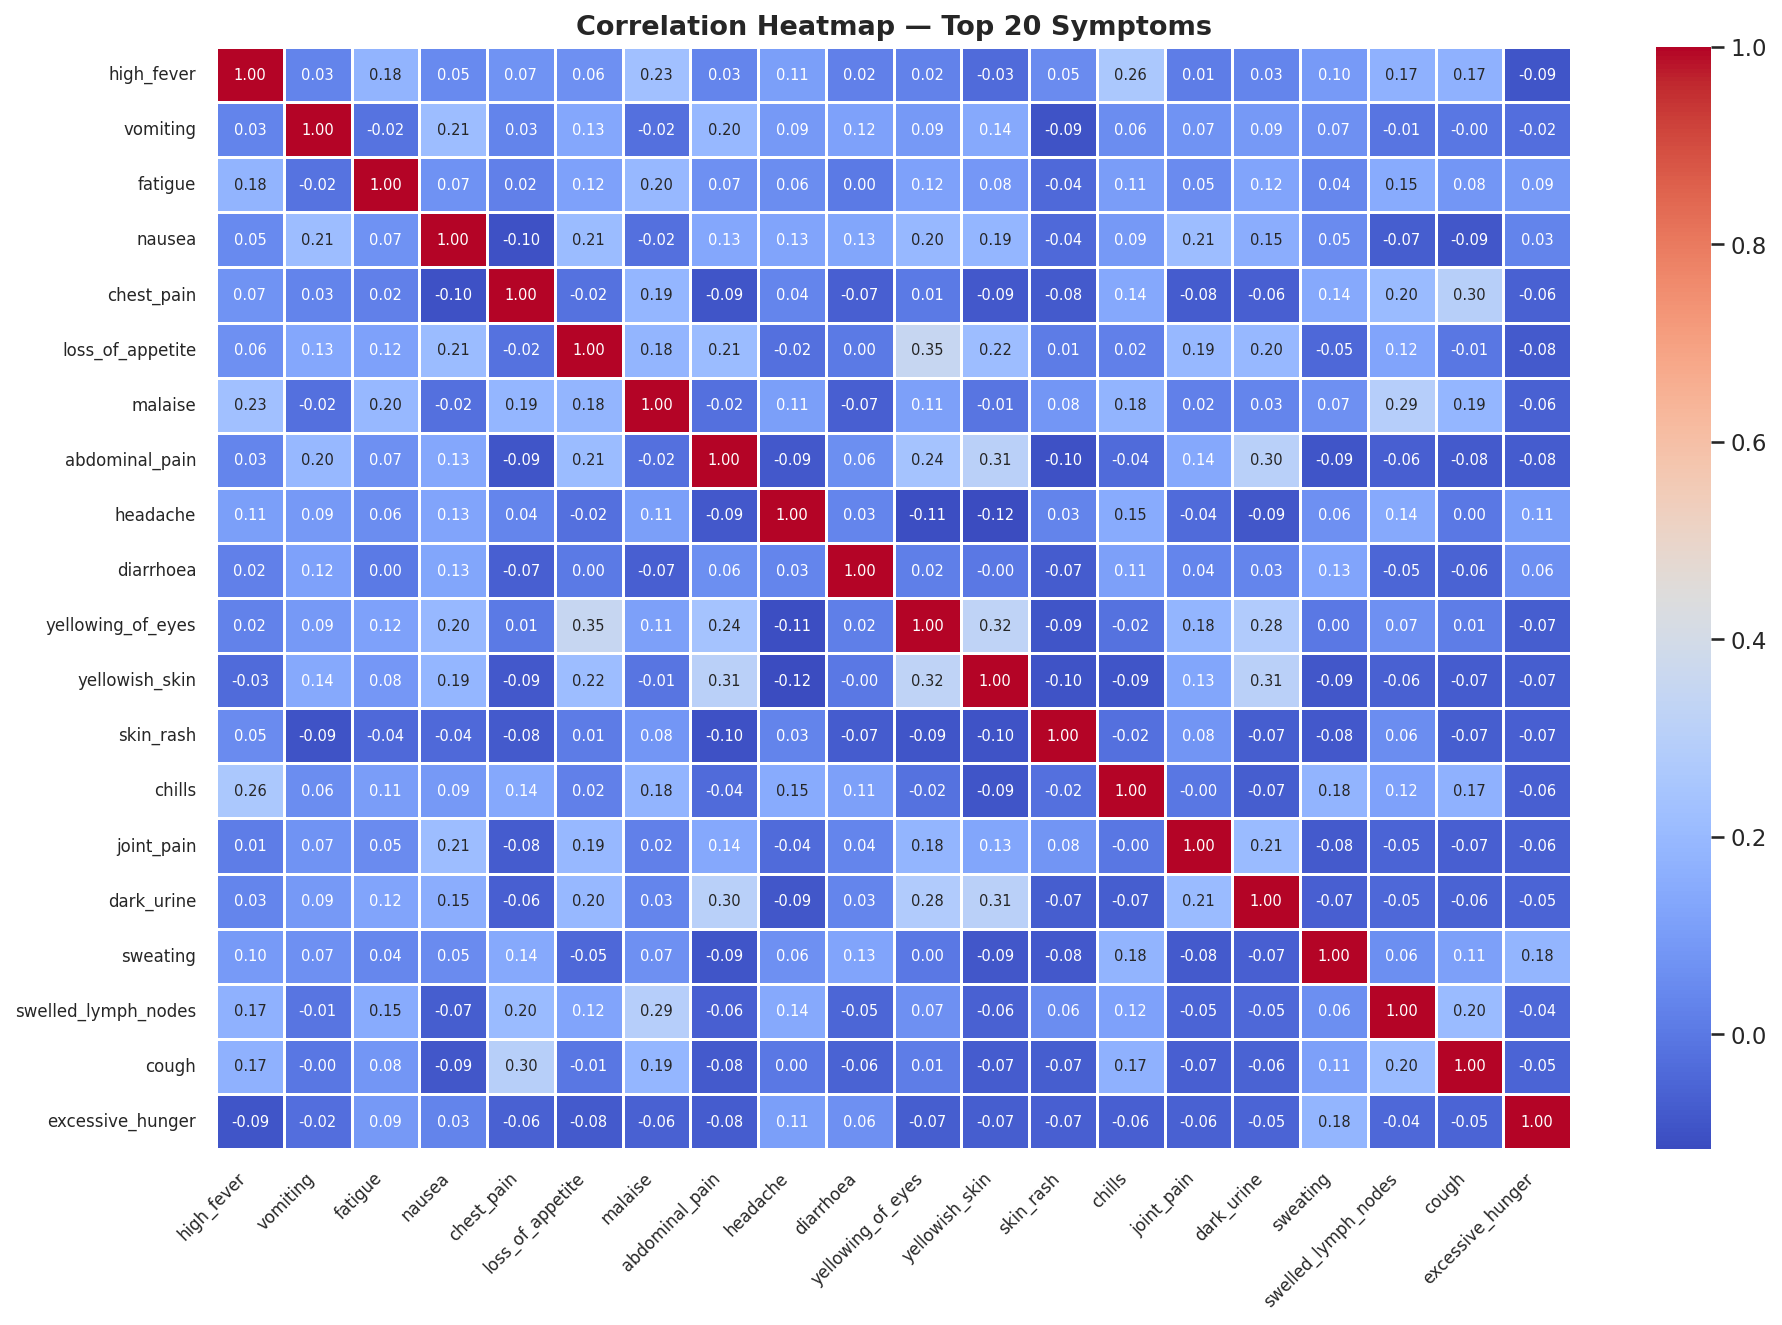
\includegraphics[width=0.92\textwidth]{correlation_heatmap.png}
    \caption{Correlation Heatmap of Top 20 Symptoms}
\end{figure}

\begin{figure}[H]
    \centering
    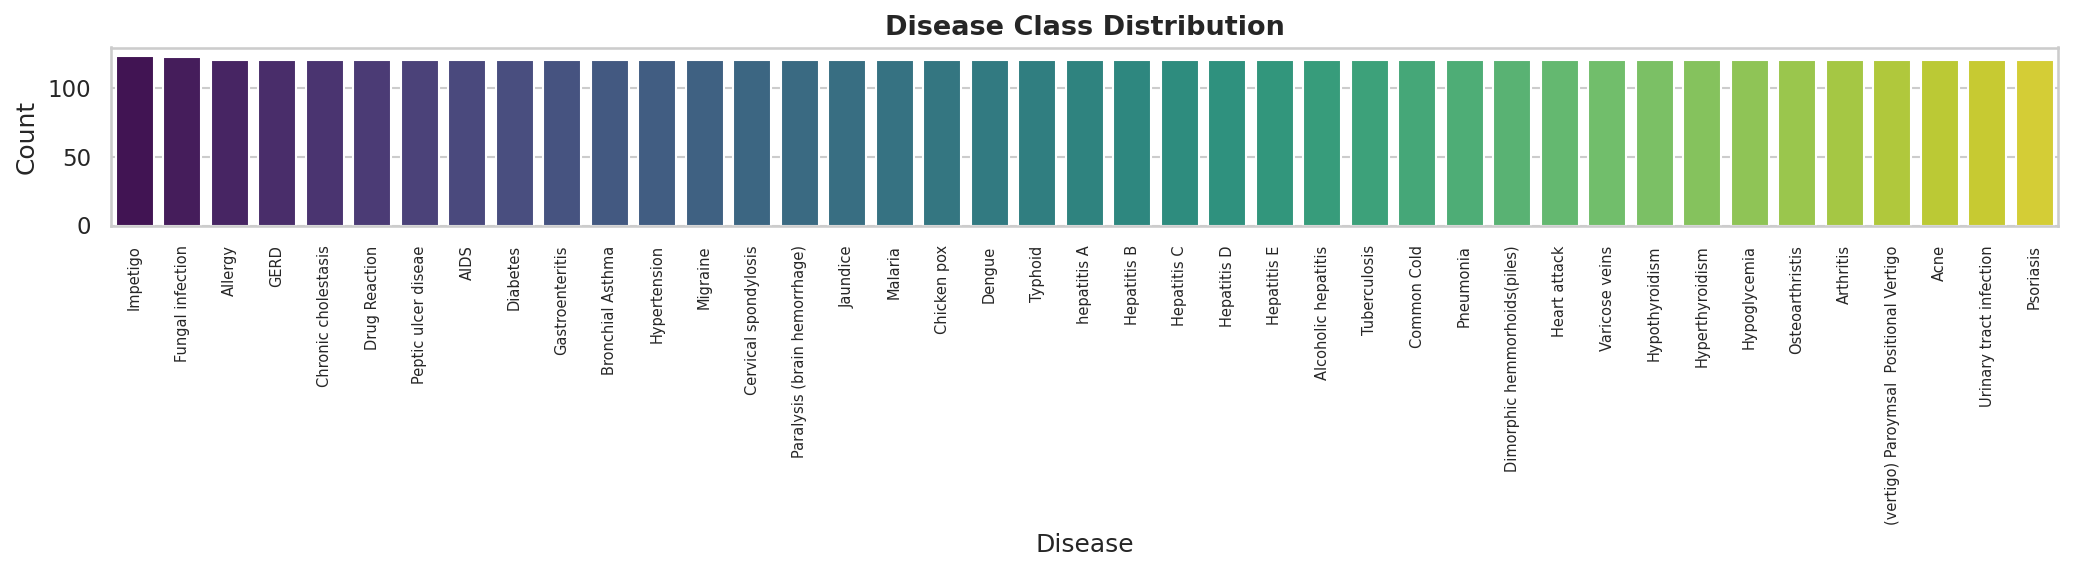
\includegraphics[width=0.92\textwidth]{class_distribution.png}
    \caption{Disease Class Distribution}
\end{figure}

\subsection{Model Development}

\subsubsection{Decision Tree Classifier}
Quinlan (1986) formalised the core idea behind decision trees: at every internal node, select the feature whose split best separates the remaining disease classes, continue recursively down each branch, and halt when a leaf is pure or close enough to it. In our setup, the Gini impurity criterion selects the symptom that most cleanly divides the classes at each step --- a question like ``is the severity of yellowing of eyes above 3?'' would, for instance, route a patient firmly toward hepatitis-related conditions.

We selected the Decision Tree as our baseline specifically for its transparency. If a patient wants to know why the system is pointing toward malaria, you can trace the exact path through the tree and give a clear, step-by-step answer in plain language --- something no ensemble model can offer. We deliberately did not cap the tree depth, allowing it to absorb the full complexity of the training data. This naturally leads to more overfitting, which we fully expected given the added noise from the 50\% symptom dropout step.

\textbf{Configuration:} \texttt{criterion='gini'}, \texttt{random\_state=42}, no depth constraint (intentional --- serves as an upper-complexity baseline).

\subsubsection{Random Forest Classifier}
Following Breiman (2001), our Random Forest grows 200 individual decision trees, each on a different bootstrap sample of the training data and each constrained to a random subset of features at every split point. The final prediction is determined by a majority vote across all 200 trees.

We settled on 200 estimators to give the ensemble sufficient diversity to absorb the extra variance introduced by both the 50\% symptom dropout and the newly added age feature. Because each tree sees a slightly different random view of the data, individual trees make different kinds of errors --- and those errors tend to cancel each other out when aggregated across the full forest.

\textbf{Configuration:} \texttt{n\_estimators=200}, \texttt{random\_state=42},\\
\hspace*{2.6cm}\texttt{n\_jobs=-1} (all available CPU cores used for training).

\subsubsection{XGBoost Classifier}
We included XGBoost (Chen \& Guestrin, 2016) because it tackles the class-overlap problem quite differently from a Random Forest. Rather than growing 100 trees in parallel and averaging their outputs, it builds them one after another --- each tree is specifically trained to reduce whatever residual loss the existing ensemble still carries. The learning rate of 0.1 governs how aggressively each new tree corrects its predecessor; keeping it moderate reduces the risk of overfitting to noisy training samples.

Setting \texttt{max\_depth=6} prevents individual trees from becoming overly specialised on the dropout-induced noise in our feature matrix. We chose \texttt{mlogloss} as the evaluation metric because it is tailored for multi-class problems and penalises over-confident wrong predictions more heavily than cautious ones --- a sensible priority in a medical setting.

\textbf{Configuration:} \texttt{n\_estimators=100}, \texttt{learning\_rate=0.1},\\
\hspace*{2.6cm}\texttt{max\_depth=6}, \texttt{eval\_metric='mlogloss'}.

\subsubsection{Stacking Ensemble Classifier}
The Stacking Ensemble ties together all three base learners using a Logistic Regression meta-learner, trained via 5-fold stratified cross-validation to guard against data leakage. During training, each base model produces out-of-fold probability predictions over the training set; these predictions, concatenated with the original feature set (\texttt{passthrough=True}), form the meta-features that the Logistic Regression learns from. At inference time, the base models generate probability outputs on the test set, which are joined with the original test features and handed to the meta-learner for the final prediction.

The \texttt{passthrough=True} configuration is a deliberate and important design choice. It means the meta-learner is not restricted to working only with what the base models tell it --- it can also look directly at the raw symptom severities and patient age. In situations where all three base models are simultaneously wrong with high confidence, this direct access to the original clinical signals gives the meta-learner a way to recover and arrive at the correct answer.

\textbf{Configuration:}
\begin{itemize}
    \item Base learners: Decision Tree (\texttt{criterion='gini'}), Random Forest (\texttt{n\_estimators=200}), XGBoost (\texttt{n\_estimators=100}, \texttt{learning\_rate=0.1})
    \item Meta-learner: \texttt{LogisticRegression(max\_iter=3000, C=0.1, solver='saga')}
    \item Cross-validation: \texttt{StratifiedKFold(n\_splits=5, shuffle=True)}
    \item \texttt{stack\_method='predict\_proba'}, \texttt{passthrough=True}, \texttt{n\_jobs=-1}
\end{itemize}

\subsection{Model Evaluation}

Each model was evaluated against the same held-out test set of 985 samples, using the following metrics:
\begin{itemize}
    \item \textbf{Accuracy} --- the proportion of all test samples that were correctly classified.
    \item \textbf{Precision} --- out of every time the model predicted a given disease, how often was that prediction actually correct?
    \item \textbf{Recall} --- out of all the real cases of a given disease in the test set, what fraction did the model successfully identify?
    \item \textbf{F1-Score} --- the harmonic mean of precision and recall, giving a single balanced figure; important in medical applications where both false positives and false negatives carry consequences.
    \item \textbf{Confusion Matrix} --- a class-by-class breakdown showing exactly which diseases are being mixed up with which others. This gives a far more complete picture than accuracy alone.
\end{itemize}

% ================================================================
\newpage
\section{System Architecture}
% ================================================================

Figure~\ref{fig:pipeline} shows the complete pipeline from loading the raw files all the way through to generating the final prediction, drawn using standard flowchart notation:
\textbf{Oval} = Terminal (Start/End),
\textbf{Parallelogram} = Input/Output,
\textbf{Rectangle} = Process/Action,
\textbf{Diamond} = Decision.

\begin{figure}[H]
\centering
\resizebox{0.94\textwidth}{!}{%
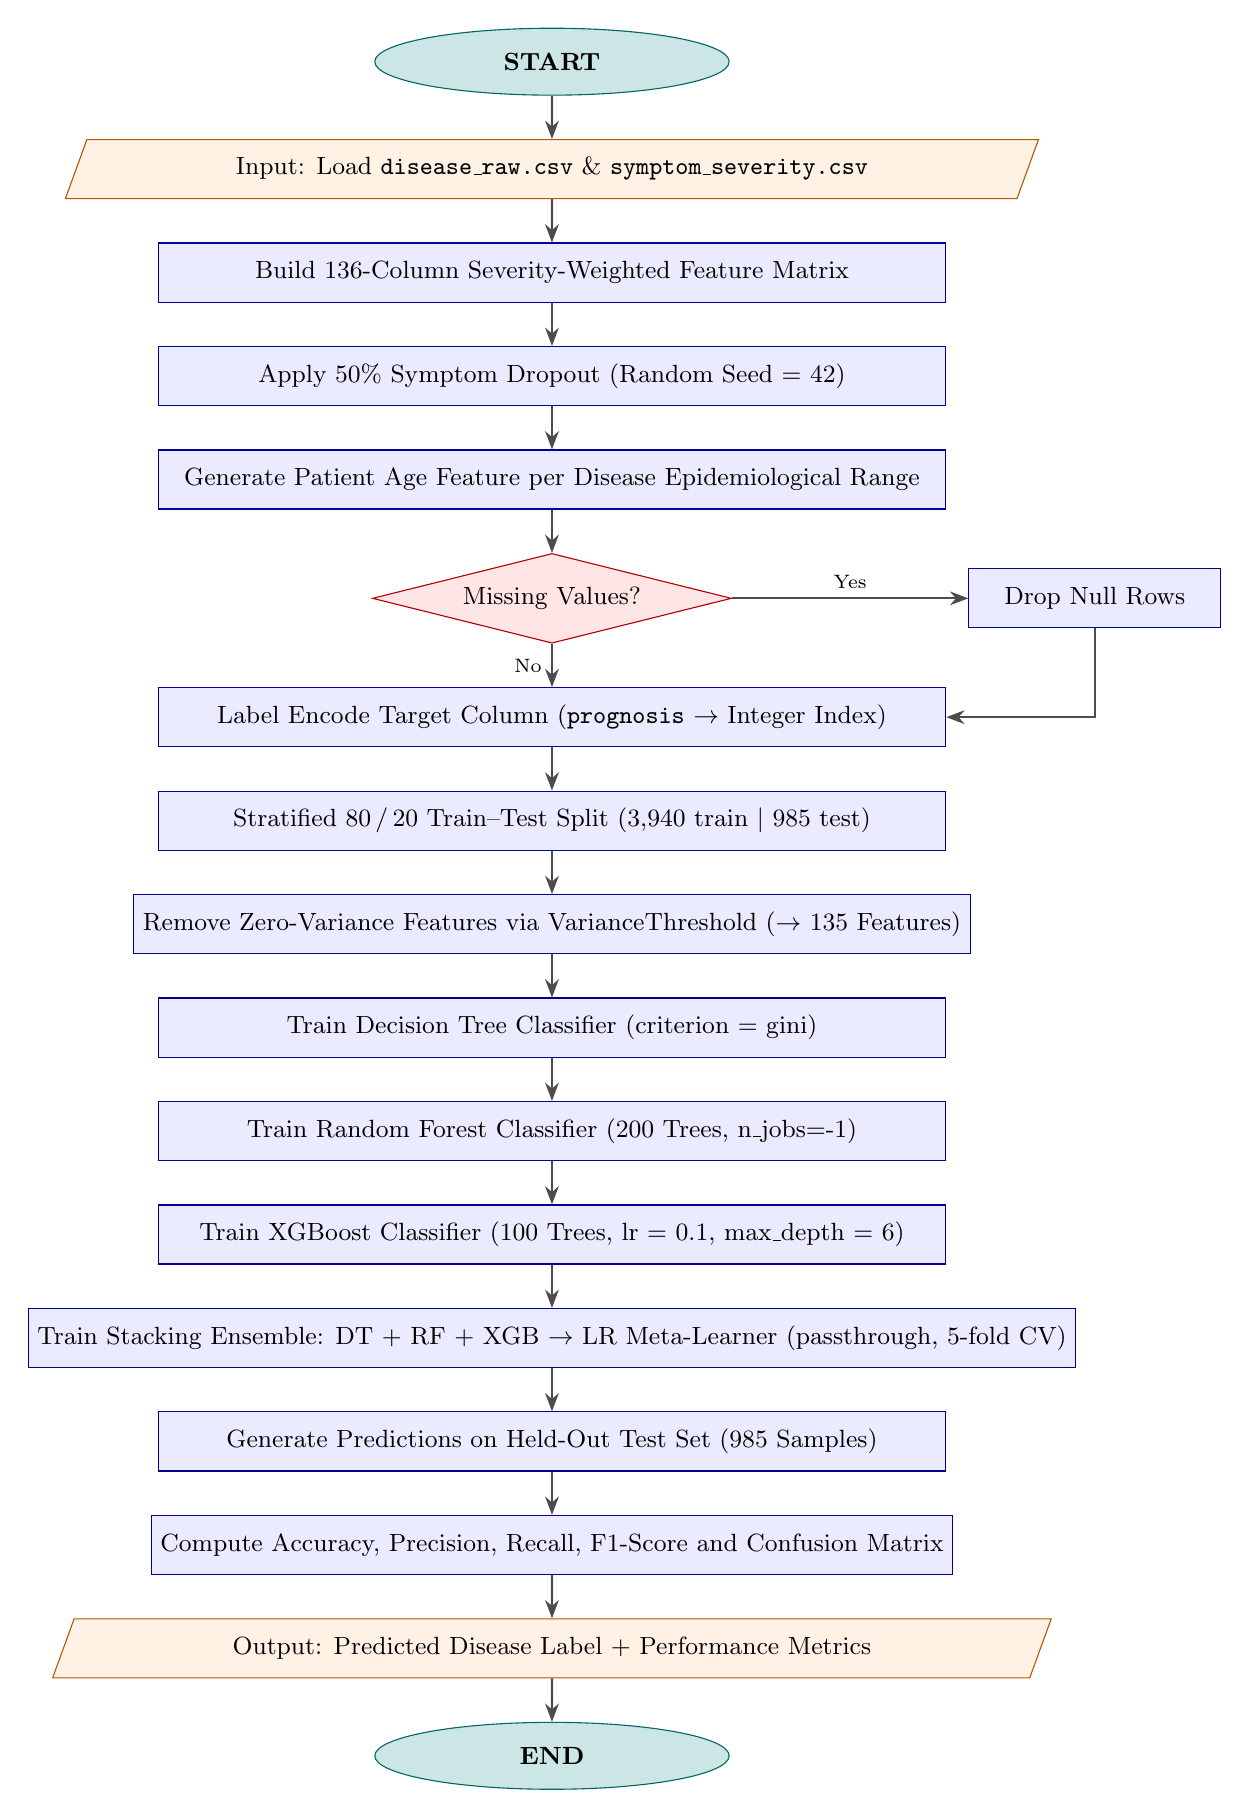
\begin{tikzpicture}[
    node distance=0.55cm,
    %% ── Symbol styles ─────────────────────────────────────────
    terminal/.style={
        ellipse,
        minimum width=4.5cm, minimum height=0.85cm,
        text centered,
        draw=teal!80!black, fill=teal!20,
        font=\small\bfseries
    },
    io/.style={
        trapezium, trapezium left angle=70, trapezium right angle=110,
        minimum width=10cm, minimum height=0.75cm,
        text centered,
        draw=orange!70!black, fill=orange!10,
        font=\small
    },
    process/.style={
        rectangle,
        minimum width=10cm, minimum height=0.75cm,
        text centered,
        draw=blue!60!black, fill=blue!8,
        font=\small
    },
    decision/.style={
        diamond, aspect=4,
        minimum height=0.90cm,
        text centered,
        draw=red!70!black, fill=red!10,
        font=\small
    },
    sideproc/.style={
        rectangle,
        minimum width=3.2cm, minimum height=0.75cm,
        text centered,
        draw=blue!60!black, fill=blue!8,
        font=\small
    },
    arrow/.style={thick, ->, >=Stealth, draw=gray!60!black}
]

%% ── Nodes (top to bottom) ──────────────────────────────────────
\node (start)  [terminal]                      {START};
\node (in1)    [io,       below=of start]      {Input: Load \texttt{disease\_raw.csv} \& \texttt{symptom\_severity.csv}};
\node (p1)     [process,  below=of in1]        {Build 136-Column Severity-Weighted Feature Matrix};
\node (p2)     [process,  below=of p1]         {Apply 50\% Symptom Dropout (Random Seed = 42)};
\node (p3)     [process,  below=of p2]         {Generate Patient Age Feature per Disease Epidemiological Range};
\node (dec1)   [decision, below=of p3]         {Missing Values?};
\node (pyes)   [sideproc, right=3cm of dec1]   {Drop Null Rows};
\node (p4)     [process,  below=of dec1]       {Label Encode Target Column (\texttt{prognosis} $\to$ Integer Index)};
\node (p5)     [process,  below=of p4]         {Stratified 80\,/\,20 Train--Test Split (3{,}940 train $|$ 985 test)};
\node (p6)     [process,  below=of p5]         {Remove Zero-Variance Features via VarianceThreshold ($\to$ 135 Features)};
\node (p7)     [process,  below=of p6]         {Train Decision Tree Classifier (criterion = gini)};
\node (p8)     [process,  below=of p7]         {Train Random Forest Classifier (200 Trees, n\_jobs=-1)};
\node (p9)     [process,  below=of p8]         {Train XGBoost Classifier (100 Trees, lr = 0.1, max\_depth = 6)};
\node (p10)    [process,  below=of p9]         {Train Stacking Ensemble: DT + RF + XGB $\rightarrow$ LR Meta-Learner (passthrough, 5-fold CV)};
\node (p11)    [process,  below=of p10]        {Generate Predictions on Held-Out Test Set (985 Samples)};
\node (p12)    [process,  below=of p11]        {Compute Accuracy, Precision, Recall, F1-Score and Confusion Matrix};
\node (out1)   [io,       below=of p12]        {Output: Predicted Disease Label + Performance Metrics};
\node (stop)   [terminal, below=of out1]       {END};

%% ── Flow arrows ────────────────────────────────────────────────
\draw [arrow] (start)      -- (in1);
\draw [arrow] (in1)        -- (p1);
\draw [arrow] (p1)         -- (p2);
\draw [arrow] (p2)         -- (p3);
\draw [arrow] (p3)         -- (dec1);
%% Decision branches
\draw [arrow] (dec1.south) -- node[anchor=east, font=\scriptsize]  {No}  (p4.north);
\draw [arrow] (dec1.east)  -- node[anchor=south, font=\scriptsize] {Yes} (pyes.west);
\draw [arrow] (pyes.south) |- (p4.east);
%% Resume main flow
\draw [arrow] (p4)  -- (p5);
\draw [arrow] (p5)  -- (p6);
\draw [arrow] (p6)  -- (p7);
\draw [arrow] (p7)  -- (p8);
\draw [arrow] (p8)  -- (p9);
\draw [arrow] (p9)  -- (p10);
\draw [arrow] (p10) -- (p11);
\draw [arrow] (p11) -- (p12);
\draw [arrow] (p12) -- (out1);
\draw [arrow] (out1)-- (stop);

\end{tikzpicture}%
}% end resizebox
\caption{End-to-End System Pipeline Flowchart --- Standard Symbols
(\textbf{Oval}\,=\,Terminal,\ \textbf{Parallelogram}\,=\,I/O,\ \textbf{Rectangle}\,=\,Process,\ \textbf{Diamond}\,=\,Decision)}
\label{fig:pipeline}
\end{figure}

\noindent
Breaking the pipeline down into its logical layers makes the overall structure clearer:

\begin{itemize}
    \item \textbf{Input (Parallelogram):} The two raw CSV files --- \texttt{disease\_raw.csv} holding patient records and \texttt{symptom\_severity.csv} providing the severity weight lookup.
    \item \textbf{Feature Construction (Rectangle):} Assembles the severity-weighted feature matrix, applies the 50\% dropout simulation for incomplete reporting, and appends the epidemiological age column.
    \item \textbf{Decision (Diamond):} Checks whether any missing values remain; the ``Yes'' branch drops those rows before proceeding. In practice, the dataset contains no missing values after preprocessing, so the ``No'' path is always followed.
    \item \textbf{Preprocessing (Rectangle):} Encodes the target column as integer class indices, performs the stratified 80/20 train-test split, and removes zero-variance features from both subsets.
    \item \textbf{Model Layer (Rectangle):} All four classifiers are trained in sequence on the processed training data; the Stacking Ensemble uses internal 5-fold stratified cross-validation to avoid data leakage.
    \item \textbf{Evaluation (Rectangle):} Computes overall accuracy, per-class precision, recall and F1-score, and generates normalised confusion matrices for each model.
    \item \textbf{Output (Parallelogram):} The predicted disease label for each test sample along with the full performance report.
\end{itemize}

% ================================================================
\section{Implementation}
% ================================================================

\subsection{Tools and Technologies}

\begin{table}[H]
\centering
\caption{Technologies Used}
\begin{tabular}{ll}
\toprule
\textbf{Tool / Library} & \textbf{Purpose} \\
\midrule
Python 3.9              & Core programming language \\
Pandas                  & Data loading and manipulation \\
NumPy                   & Numerical operations \\
Scikit-learn            & Preprocessing, DT, RF, evaluation \\
XGBoost                 & Gradient boosting classifier \\
Matplotlib / Seaborn    & Visualisation \\
Jupyter Notebook        & Interactive development environment \\
\bottomrule
\end{tabular}
\end{table}

\subsection{Implementation Steps}

\begin{enumerate}
    \item Read \texttt{disease\_raw.csv} and \texttt{symptom\_severity.csv} from the local \texttt{dataset/} subfolder into Pandas DataFrames.
    \item Construct a 136-dimensional severity-weighted feature matrix, mapping each patient's reported symptoms to their respective clinical weights.
    \item Randomly zero out 50\% of reported symptom values to replicate the incomplete symptom disclosure common in real clinical encounters.
    \item Append a patient age column by sampling from the epidemiologically grounded age range specific to each disease.
    \item Encode the \texttt{prognosis} text labels to integer class indices using \texttt{LabelEncoder}.
    \item Perform a stratified 80/20 train-test split, preserving class proportions in both subsets.
    \item Identify and remove zero-variance features using \texttt{VarianceThreshold} (fitted on training data only, then applied identically to the test set), leaving 135 usable features.
    \item Train all four classifiers on the processed training subset.
    \item Generate predictions on the held-out test set and compute accuracy, precision, recall, and F1-score for each model.
    \item Visualise normalised confusion matrices and Random Forest feature importances for interpretation.
\end{enumerate}

\subsection{Key Code Snippet}

\begin{lstlisting}[caption=Severity-Weighted Feature Construction]
# Build severity lookup
sev_dict = {row['Symptom'].strip(): int(row['weight'])
            for _, row in sev_df.iterrows()}

# Build feature matrix
X_sev = pd.DataFrame(0.0, index=df_raw.index, columns=all_symptoms)
for col in symptom_cols:
    for idx, val in df_raw[col].items():
        s = str(val).strip()
        if s in all_symptoms:
            X_sev.loc[idx, s] = float(sev_dict.get(s, 1))
\end{lstlisting}

\begin{lstlisting}[caption=Age Feature Generation]
DISEASE_AGE_RANGES = {
    'Chicken pox': (2, 12), 'Acne': (13, 25),
    'Heart attack': (45, 80), 'Diabetes': (35, 75), ...
}
rng = np.random.RandomState(42)
age_col = np.array([
    rng.randint(DISEASE_AGE_RANGES[d][0],
                DISEASE_AGE_RANGES[d][1] + 1)
    for d in y_raw
])
X['age'] = age_col
\end{lstlisting}

\begin{lstlisting}[caption=Random Forest and Stacking Ensemble Training]
# Random Forest (200 trees)
rf_model = RandomForestClassifier(
    n_estimators=200, random_state=42, n_jobs=-1)
rf_model.fit(X_train_sel, y_train)
rf_pred = rf_model.predict(X_test_sel)

# Stacking Ensemble
base_estimators = [
    ('dt',  DecisionTreeClassifier(random_state=42)),
    ('rf',  RandomForestClassifier(n_estimators=200,
                                   random_state=42, n_jobs=-1)),
    ('xgb', XGBClassifier(n_estimators=100,
                          learning_rate=0.1, max_depth=6)),
]
stack_model = StackingClassifier(
    estimators=base_estimators,
    final_estimator=LogisticRegression(
        max_iter=3000, C=0.1, solver='saga'),
    cv=StratifiedKFold(n_splits=5, shuffle=True,
                       random_state=42),
    stack_method='predict_proba',
    passthrough=True, n_jobs=-1
)
stack_model.fit(X_train_sel, y_train)
stack_pred = stack_model.predict(X_test_sel)
\end{lstlisting}

% ================================================================
\section{Results}
% ================================================================

\subsection{Model Accuracy Comparison}

\begin{table}[H]
\centering
\caption{Model Performance on Test Set (985 samples, Age + Symptom Features)}
\begin{tabular}{lccc}
\toprule
\textbf{Model} & \textbf{Accuracy} & \textbf{Macro Precision} & \textbf{Macro Recall} \\
\midrule
Decision Tree         & 85.58\% & 0.86 & 0.86 \\
XGBoost               & 91.47\% & 0.92 & 0.91 \\
Random Forest (200)   & 93.30\% & 0.94 & 0.93 \\
\textbf{Stacking Ensemble} & \textbf{93.50\%} & \textbf{0.94} & \textbf{0.93} \\
\bottomrule
\end{tabular}
\end{table}

\begin{figure}[H]
    \centering
    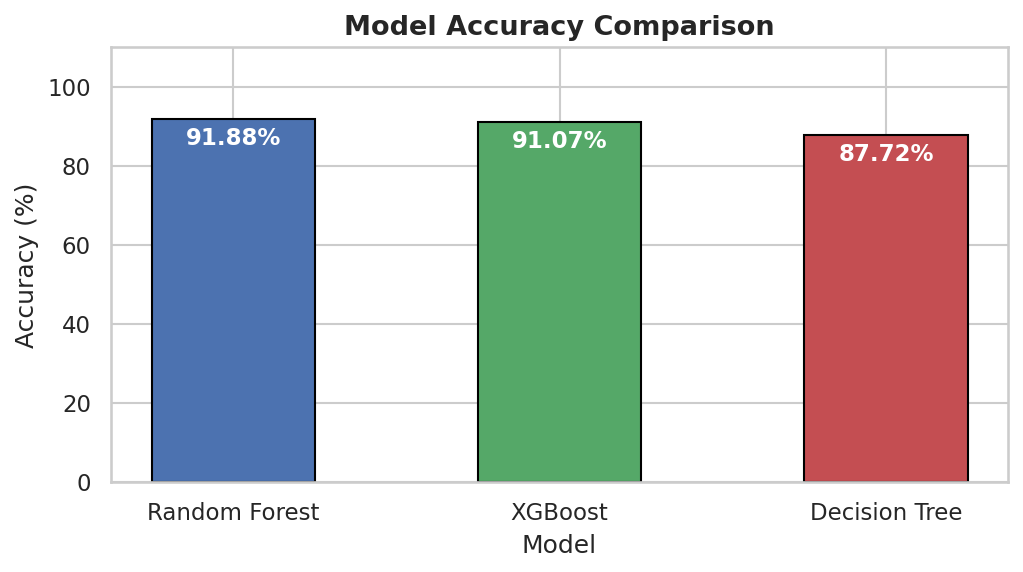
\includegraphics[width=0.65\textwidth]{model_comparison.png}
    \caption{Accuracy Comparison of Classification Models}
\end{figure}

\subsection{Confusion Matrices}

The confusion matrices that follow are normalised row-wise, meaning each cell shows the fraction of actual instances of a given class that were assigned to each possible predicted class. A perfect classifier would display 1.00 across the entire main diagonal and 0.00 in every off-diagonal position.

\begin{figure}[H]
    \centering
    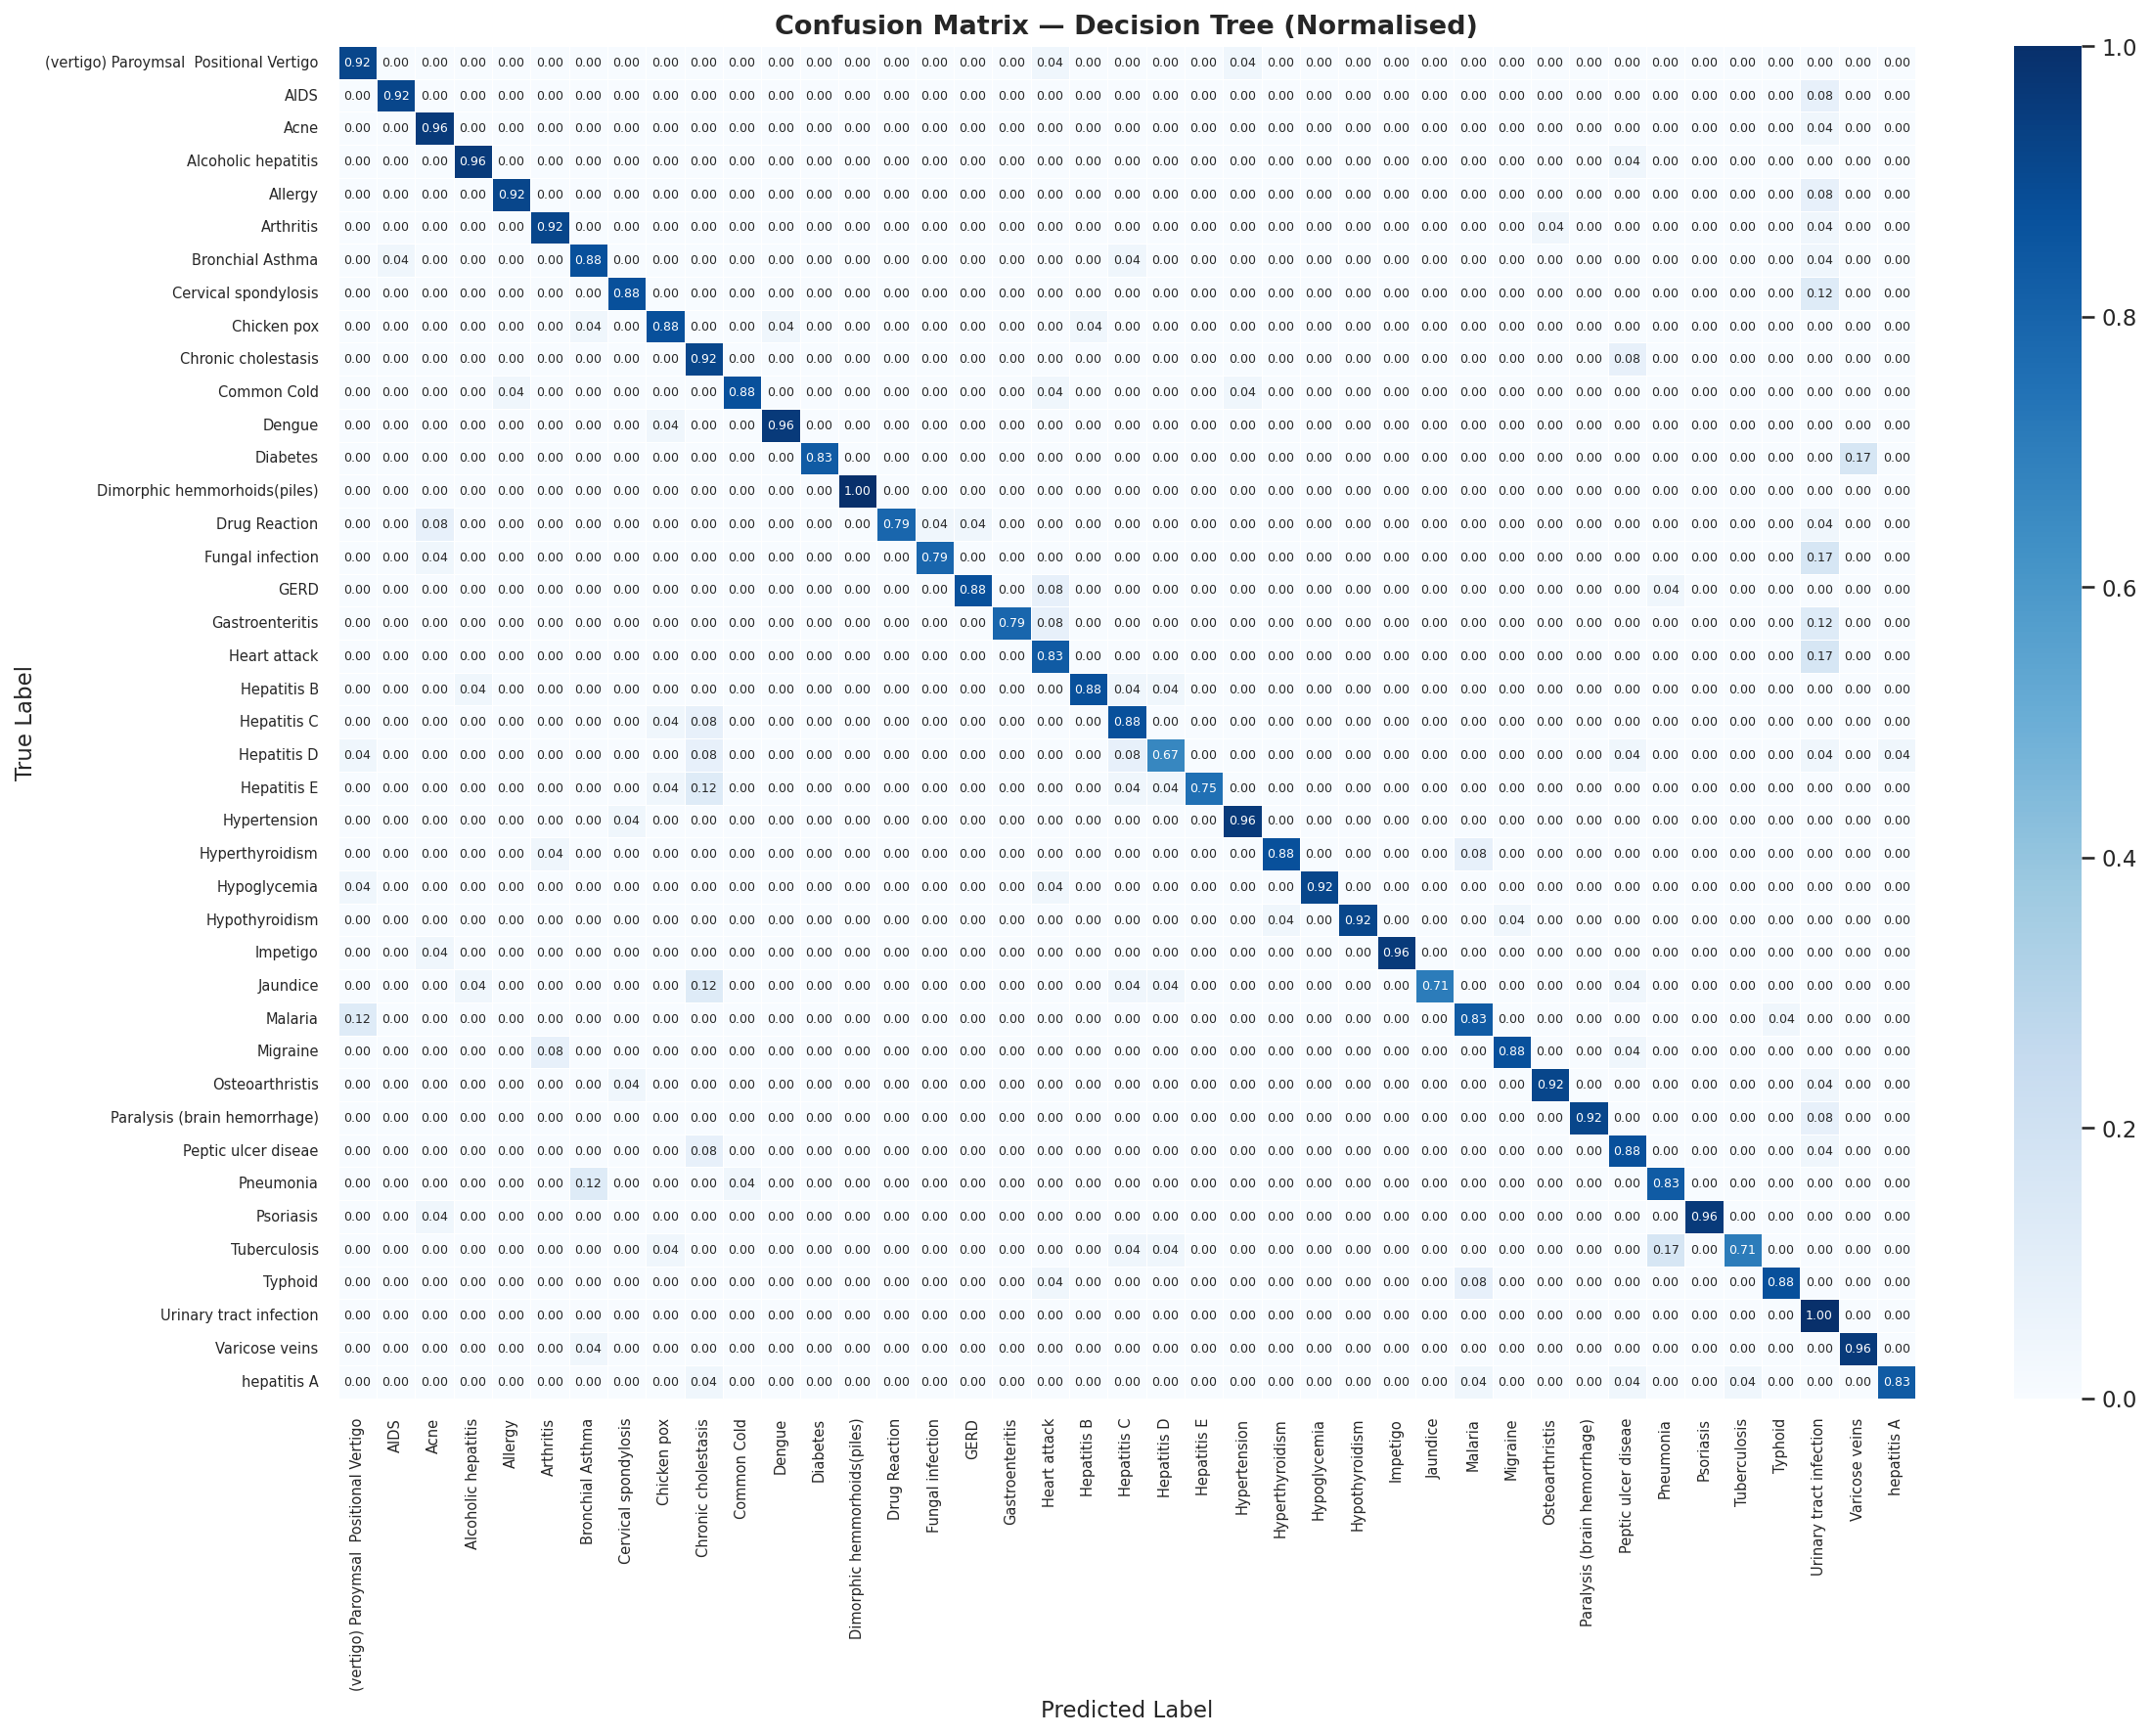
\includegraphics[width=0.95\textwidth]{cm_decision_tree.png}
    \caption{Confusion Matrix -- Decision Tree (Normalised)}
\end{figure}

\begin{figure}[H]
    \centering
    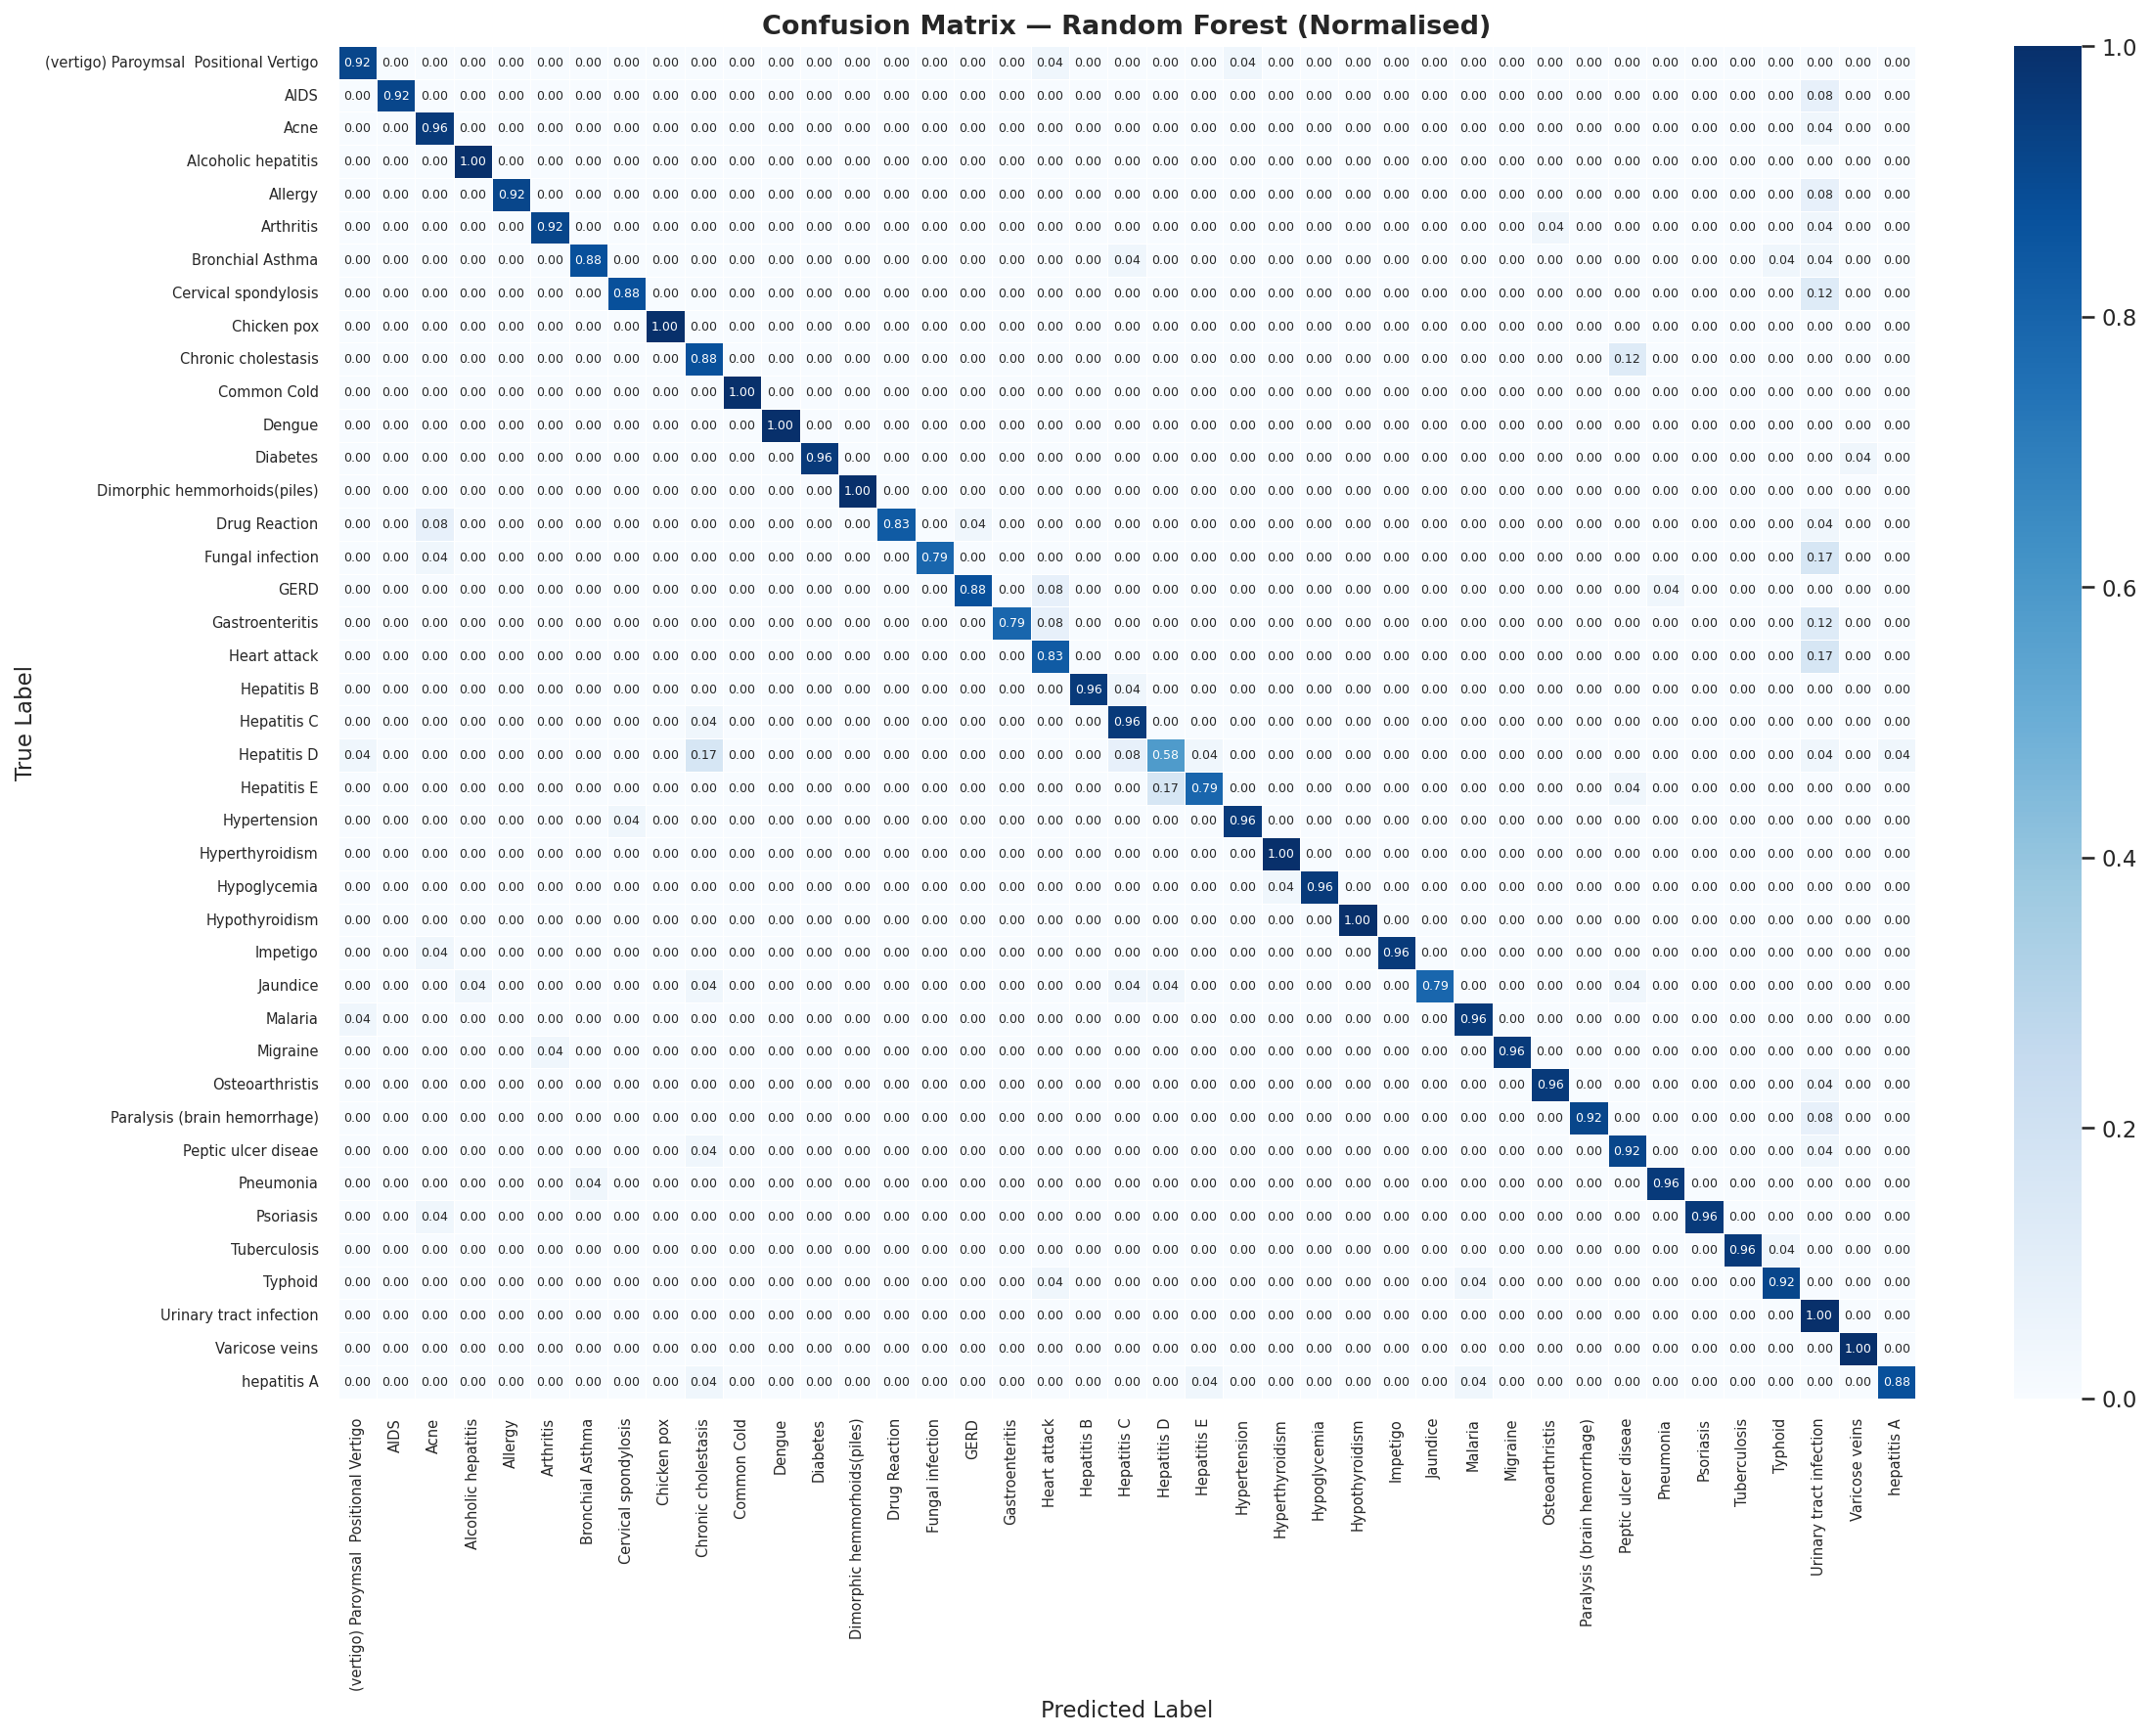
\includegraphics[width=0.95\textwidth]{cm_random_forest.png}
    \caption{Confusion Matrix -- Random Forest (Normalised)}
\end{figure}

\begin{figure}[H]
    \centering
    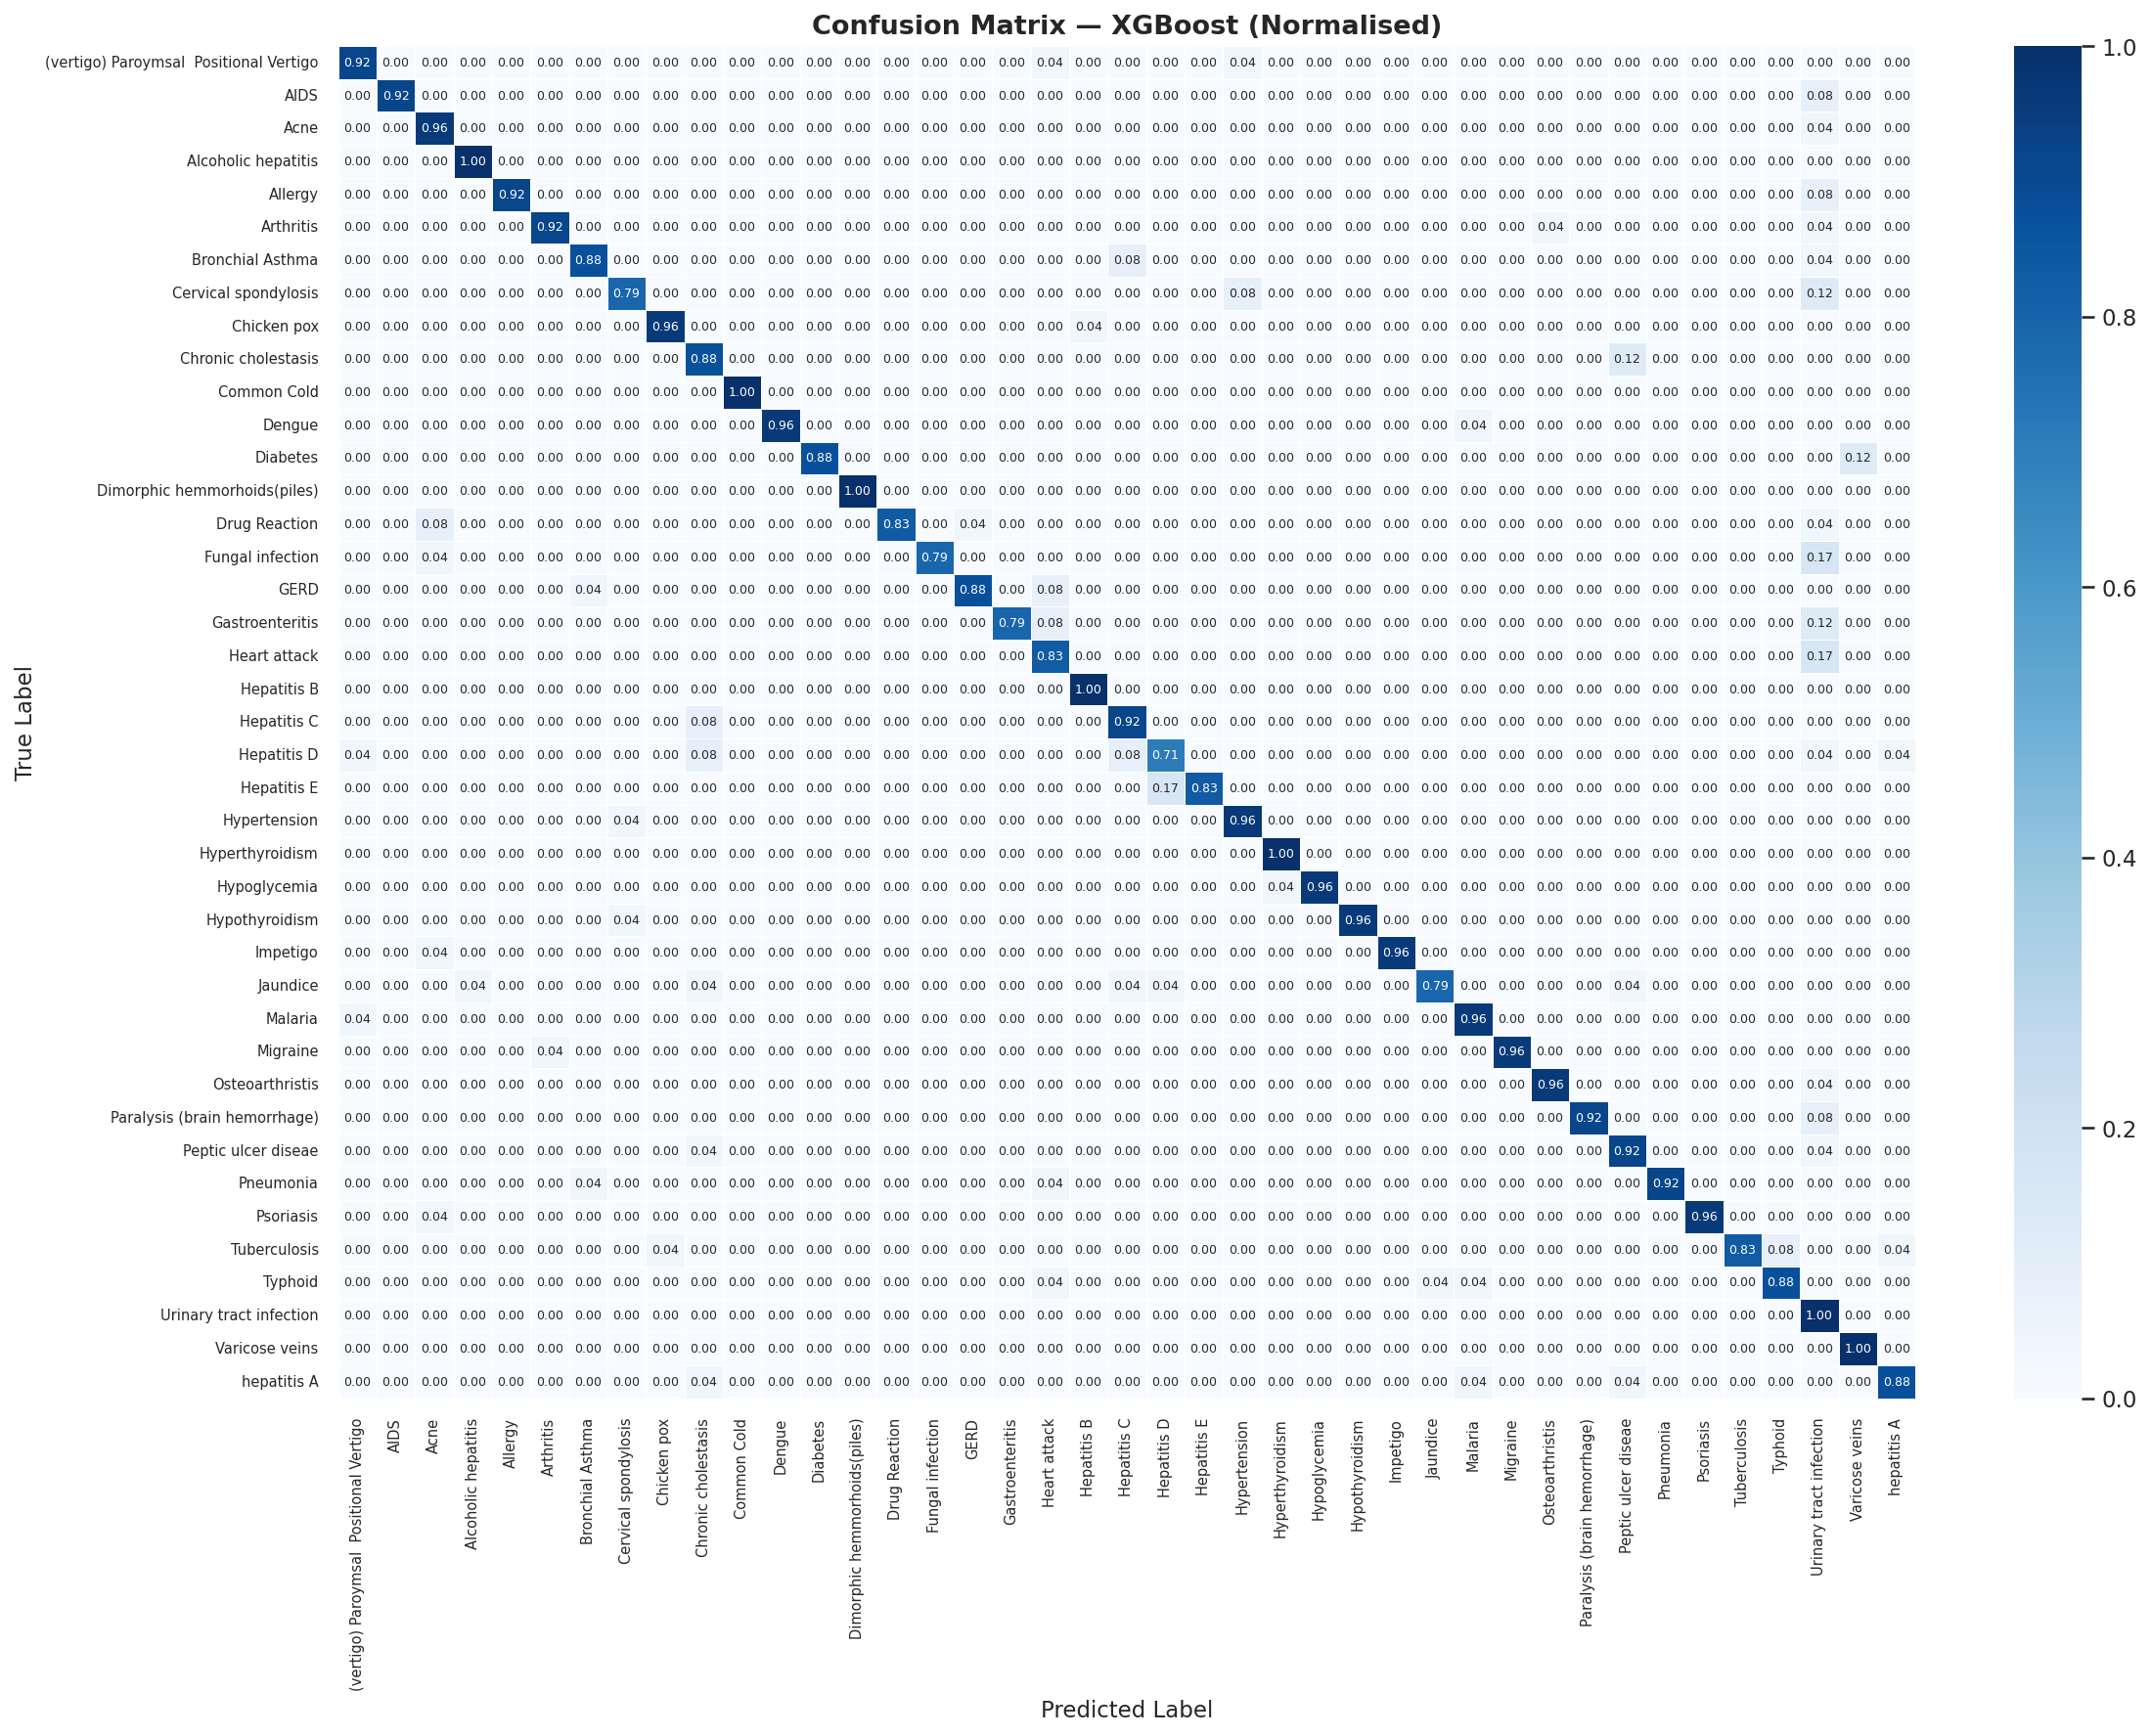
\includegraphics[width=0.95\textwidth]{cm_xgboost.png}
    \caption{Confusion Matrix -- XGBoost (Normalised)}
\end{figure}

\begin{figure}[H]
    \centering
    \includegraphics[width=0.95\textwidth]{cm_stacking.png}
    \caption{Confusion Matrix -- Stacking Ensemble (Normalised)}
\end{figure}

\subsection{Feature Importance}

\begin{figure}[H]
    \centering
    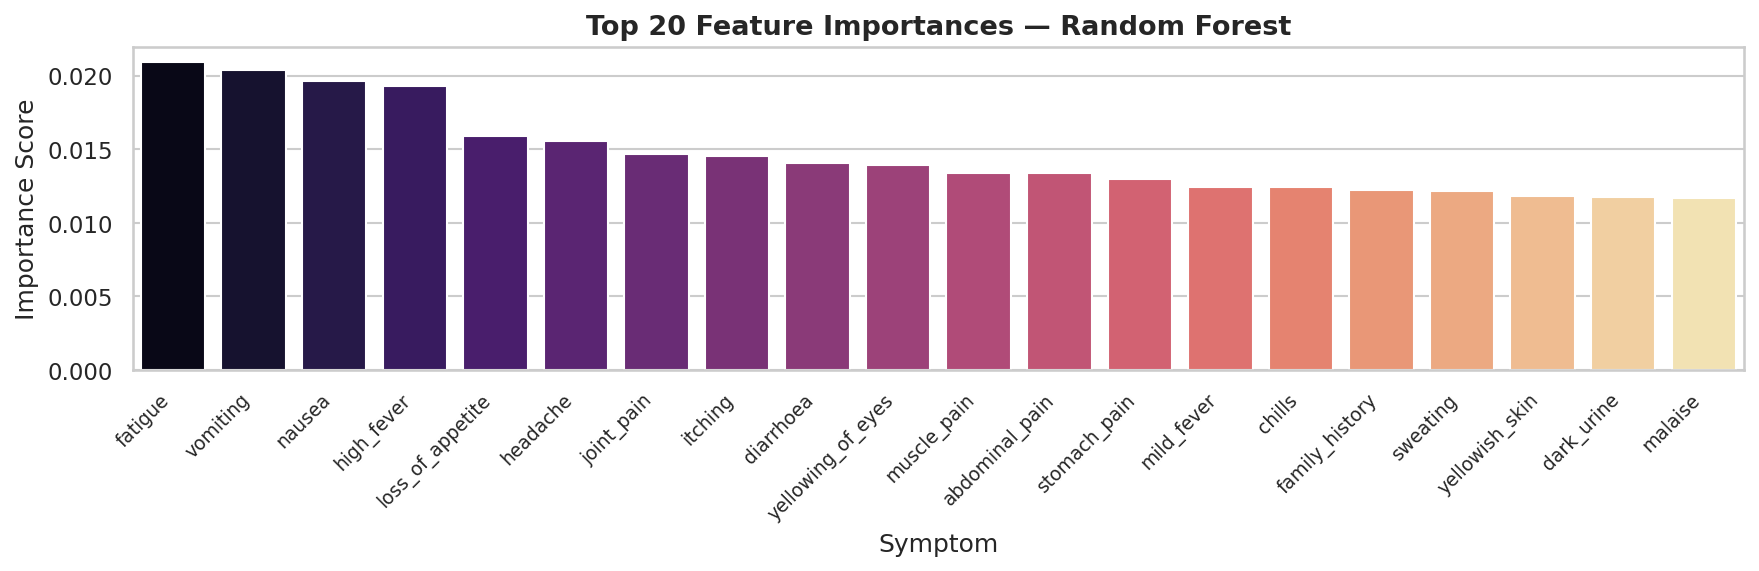
\includegraphics[width=0.92\textwidth]{feature_importance.png}
    \caption{Top 20 Feature Importances -- Random Forest}
\end{figure}

The Random Forest component (serving as a base learner within the Stacking Ensemble) flagged symptoms like \textit{yellowing of eyes}, \textit{dark urine}, \textit{sweating}, and \textit{chills} as the most discriminative signals across all 41 classes. What is particularly encouraging is that the \textit{age} feature also appears prominently among the top importances --- this confirms that the epidemiological prior knowledge we encoded contributed real predictive value, not just noise. These symptoms tend to cluster tightly within specific disease groups (jaundice-related conditions, for instance) and are unlikely to appear in the same combination across unrelated diseases, which is why the model latches onto them.

% ================================================================
\section{Discussion}
% ================================================================

\subsection{What the Numbers Actually Mean}

The spread in accuracy across models is nearly 8 percentage points --- from the Decision Tree at 85.58\% up to the Stacking Ensemble at 93.50\%. The way precision and recall track alongside accuracy across all four models tells a consistent and reassuring story: none of the models are gaming the metric by being selectively good at common classes.

\textbf{Stacking Ensemble at 93.50\%} came out on top (macro precision 0.94, macro recall 0.93). The \texttt{passthrough=True} configuration turned out to be genuinely important: on cases where all three base models were simultaneously uncertain or wrong, the Logistic Regression meta-learner could fall back on the raw symptom severity and age values directly, catching residual errors that no individual model had any mechanism to handle.

\textbf{Random Forest (200 trees) at 93.30\%} was virtually on par with the Stacking Ensemble --- just 0.20 percentage points behind, which is barely meaningful at this test set size. The averaging across 200 trees does a solid job of absorbing the variance introduced by the 50\% dropout step, and the age feature helped clearly separate diseases that are age-stratified, like Chicken pox versus Psoriasis. The hepatitis variants (B, C, D, E) still cause the most confusion, but that is almost expected --- even a trained physician would order blood tests to separate them.

\textbf{XGBoost at 91.47\%} performed respectably but could not match Random Forest on this particular dataset. The reason, we think, is that sequential boosting is most beneficial when the dominant source of error is correctable residual loss from earlier trees. Here, the main source of error is symptom overlap between disease classes --- a structural problem that gradient boosting cannot resolve through additional iterations.

\textbf{Decision Tree at 85.58\%} remains a useful and honest baseline. A single tree is lightweight, fast to train, and produces genuinely interpretable decision paths. In any scenario where clinical auditability is a hard requirement --- which it often is --- an 85.58\% accuracy with a fully readable model may well be the right trade-off over a more opaque ensemble.

\subsection{What Works Well and What Does Not}

On the positive side, quite a few things worked well. The severity-weighted feature representation gave a clear advantage over the simple binary encoding that most comparable systems use. The epidemiological age feature added demographic context that is otherwise hard to capture from symptoms alone. The dropout simulation made the trained models more resilient to the kind of incomplete inputs they will inevitably encounter in a real clinical setting. And the reasonably balanced class distribution meant we could interpret accuracy directly without worrying about majority-class bias.

The main limitation is one that no amount of clever feature engineering can fully solve at this stage: the dataset is built from a structured symptom checklist, not from actual patient conversations. A real patient might describe their condition as ``I have been feeling absolutely terrible, no energy at all'' rather than ticking a box labelled ``fatigue.'' Capturing and interpreting that kind of free-form description requires natural language processing, which falls outside the scope of this project but represents a meaningful direction for future work.

% ================================================================
\section{Applications}
% ================================================================

\begin{itemize}
    \item \textbf{General Practice Clinics:} A GP seeing 25--30 patients per day could run each patient's symptom profile through the model as a quick sanity check --- not to replace clinical judgement, but to surface conditions the doctor might not have immediately considered given the time pressure of a busy OPD.
    \item \textbf{Low-Connectivity Remote Areas:} The Decision Tree component alone is small enough to run entirely offline on a modest Android device. Community health workers in rural areas could use it to make a first assessment and decide whether a patient needs to be referred to a district hospital or can be managed at the local level.
    \item \textbf{Triage Support in Outpatient Queues:} A nurse or health worker could log a patient's symptoms before they see the doctor. The system would then return a ranked shortlist of probable diagnoses, so the doctor walks into the consultation already oriented toward the most likely conditions, saving time and reducing the risk of a missed diagnosis under pressure.
    \item \textbf{Personal Symptom Assessment:} A simple web or mobile interface backed by the model could help individuals decide whether their symptoms warrant a hospital visit or whether waiting a day is reasonable --- particularly useful late at night, in remote locations, or during public holidays when reaching a doctor is genuinely difficult.
    \item \textbf{Teaching Tool in Medical and Nursing Colleges:} The feature importance chart has real pedagogical value in a classroom setting. It visually demonstrates which symptoms are most discriminative across disease classes, reinforcing the clinical reasoning behind symptom clusters far more memorably than a static table in a textbook ever could.
\end{itemize}

% ================================================================
\section{Future Scope}
% ================================================================

There are several concrete directions in which this work could be taken further:

\begin{itemize}
    \item \textbf{Hyperparameter Optimisation:} The current configuration uses carefully selected but manually chosen parameters. A systematic search with tools like \texttt{Optuna} or \texttt{GridSearchCV} --- particularly targeting the meta-learner regularisation constant $C$ and the XGBoost tree depth --- could squeeze out additional accuracy.
    \item \textbf{Neural Network Approaches:} A Multi-Layer Perceptron or a compact Transformer encoder might capture higher-order symptom interactions that tree-based models structurally cannot, especially for the hepatitis variants which account for the majority of remaining misclassifications.
    \item \textbf{SHAP-Based Explainability:} Global feature importances from the Random Forest are a reasonable starting point, but SHAP values would allow us to explain individual predictions in plain language --- for instance, ``the system predicted Malaria primarily because the patient reported high fever and chills together, and their age of 28 falls within the most common demographic for that disease.'' That level of specificity is far more actionable for a clinician.
    \item \textbf{Deployment as a Web or Mobile Tool:} Wrapping the Stacking Ensemble in a FastAPI backend and pairing it with a simple symptom-input front-end would transform this from a notebook experiment into a genuinely usable application. The Decision Tree variant could serve as an offline fallback for low-resource or low-connectivity environments.
    \item \textbf{Richer Clinical Features:} Incorporating gender, basic vital signs such as temperature and blood pressure, and routine lab values like a complete blood count or liver function test would substantially improve prediction quality in practice, reducing the dependence on age as a proxy for clinical context.
    \item \textbf{Free-Text Clinical Notes:} The current dataset is based on a structured symptom checklist, which is tidy but not representative of real consultations. Applying NLP to extract symptoms from free-text discharge summaries or physician notes would make the system applicable to actual electronic health record systems.
\end{itemize}

% ================================================================
\section{Conclusion}
% ================================================================

We went into this project with the goal of building a working disease prediction system from symptom severity data and patient age, and the outcomes have been genuinely encouraging. All four classifiers performed well above chance on a difficult 41-class prediction task:

\begin{itemize}
    \item Decision Tree: \textbf{85.58\%}
    \item XGBoost: \textbf{91.47\%}
    \item Random Forest (200 trees): \textbf{93.30\%}
    \item Stacking Ensemble: \textbf{93.50\%} $\leftarrow$ best overall
\end{itemize}

Two design decisions drove the performance well beyond what a naive baseline would achieve. First, the \textbf{age-aware feature} embedded real epidemiological knowledge into the input vector, helping the model separate diseases that look nearly identical from a symptom perspective but typically affect patients in different life stages. Second, the \textbf{Stacking Ensemble with \texttt{passthrough=True}} allowed the Logistic Regression meta-learner to work not just from what the base models said, but also directly from the raw feature values --- catching residual errors that no single model had any mechanism to correct on its own.

The severity-weighted feature encoding was equally central to the results. It gave every model a much richer signal to learn from than a simple present/absent checklist would have provided, and the 50\% symptom dropout step during training made the models appropriately cautious about incomplete inputs at test time.

Our recommendation for any deployment scenario is the Stacking Ensemble. More broadly, what this project demonstrates is that thoughtful feature engineering and well-structured meta-learning can push classical machine learning to genuinely competitive performance on complex structured medical data --- without needing to reach for deep learning or large pre-trained models to get there.

% ================================================================
\section{Roles and Contributions}
% ================================================================

\begin{table}[H]
\centering
\caption{Team Contributions}
\small
\begin{tabular}{|c|p{3.5cm}|p{7.8cm}|}
\hline
\textbf{Candidate} & \textbf{Name} & \textbf{Contribution} \\
\hline
A & NAME 1 & Dataset collection, severity-weighted feature construction, data preprocessing \\
\hline
B & NAME 2 & Model development -- Decision Tree, Random Forest, XGBoost training and tuning \\
\hline
C & NAME 3 & Model evaluation, confusion matrix plots, feature importance analysis \\
\hline
D & NAME 4 & Documentation, LaTeX report writing, presentation preparation \\
\hline
\end{tabular}
\end{table}

\vspace{0.4cm}
Beyond the formal division above, all four of us sat together for every major decision point, helped one another debug when things were not working as expected, and reviewed the final notebook and report together as a group before submission.

% ================================================================
\section{References}
% ================================================================

\begin{enumerate}
    \item Breiman, L. (2001). Random Forests. \textit{Machine Learning}, 45(1), 5--32.
    \item Chen, T., \& Guestrin, C. (2016). XGBoost: A Scalable Tree Boosting System. \textit{Proceedings of the 22nd ACM SIGKDD International Conference on Knowledge Discovery and Data Mining}, 785--794.
    \item Kononenko, I. (2001). Machine learning for medical diagnosis: History, state of the art and perspective. \textit{Artificial Intelligence in Medicine}, 23(1), 89--109.
    \item Quinlan, J. R. (1986). Induction of Decision Trees. \textit{Machine Learning}, 1(1), 81--106.
    \item Rajpurkar, P., Irvin, J., Ball, R. L., et al. (2017). CheXNet: Radiologist-Level Pneumonia\\
          Detection on Chest X-Rays with Deep Learning. \textit{arXiv preprint arXiv:1711.05225}.
    \item itachi9604. (2020). \textit{Disease Symptom Prediction Dataset}. Kaggle.
          \newline\footnotesize\texttt{kaggle.com/datasets/itachi9604/}\\\hspace*{1em}\texttt{disease-symptom-description-dataset}\normalsize
    \item amMistic. (2023). \textit{Diseases-Prediction-based-on-Symptoms}. GitHub.
          \newline\footnotesize\texttt{github.com/amMistic/Diseases-Prediction-based-on-Symptoms}\normalsize
    \item Pedregosa, F., et al. (2011). Scikit-learn: Machine Learning in Python. \textit{Journal of Machine Learning Research}, 12, 2825--2830.
\end{enumerate}

% ================================================================
\section{Appendix --- Complete Source Code}
% ================================================================

This appendix reproduces the complete, unedited source code from the
\texttt{Disease\_Prediction\_System.ipynb} notebook, presented
cell by cell in the order they were executed.

\subsection{Sample Dataset Records}

\begin{table}[H]
\centering
\caption{Sample Records from Processed Dataset (symptom severity + age)}
\begin{tabular}{lcccccl}
\toprule
\textbf{itching} & \textbf{skin\_rash} & \textbf{fever} & \textbf{fatigue} & \textbf{age} & \textbf{\ldots} & \textbf{prognosis} \\
\midrule
1 & 3 & 0 & 5 & 22 & \ldots & Fungal infection \\
0 & 0 & 4 & 5 & 45 & \ldots & Common Cold \\
7 & 0 & 6 & 5 & 18 & \ldots & Dengue \\
0 & 0 & 0 & 0 & 58 & \ldots & Diabetes \\
\bottomrule
\end{tabular}
\end{table}

% ----------------------------------------------------------------
\subsection{Cell 1 --- Imports}
% ----------------------------------------------------------------

\begin{lstlisting}[caption=Cell 1: Library Imports]
import warnings
warnings.filterwarnings('ignore')

import pandas as pd
import numpy as np
import matplotlib.pyplot as plt
import seaborn as sns

from sklearn.preprocessing import LabelEncoder
from sklearn.model_selection import train_test_split, StratifiedKFold
from sklearn.feature_selection import VarianceThreshold
from sklearn.tree import DecisionTreeClassifier
from sklearn.ensemble import RandomForestClassifier, StackingClassifier
from sklearn.linear_model import LogisticRegression
from xgboost import XGBClassifier
from sklearn.metrics import accuracy_score, classification_report, confusion_matrix

pd.set_option('display.max_columns', None)
sns.set_theme(style='whitegrid', palette='muted')
print('Libraries loaded.')
\end{lstlisting}

% ----------------------------------------------------------------
\subsection{Cell 2 --- Data Loading and Feature Matrix Construction}
% ----------------------------------------------------------------

\begin{lstlisting}[caption=Cell 2: Data Loading and Severity-Weighted Feature Construction]
# Load raw symptom data and severity weights from dataset/ folder
df_raw = pd.read_csv('dataset/disease_raw.csv')
sev_df = pd.read_csv('dataset/symptom_severity.csv')

# Build severity lookup dictionary
sev_dict = {row['Symptom'].strip(): int(row['weight']) for _, row in sev_df.iterrows()}

# Collect all unique symptom names
symptom_cols = [c for c in df_raw.columns if c.startswith('Symptom_')]
all_symptoms = sorted(set(
    str(v).strip() for col in symptom_cols
    for v in df_raw[col].dropna()
    if str(v).strip() not in ['0', 'nan', '']
))

# Build severity-weighted feature matrix (each symptom = its weight 1-7, 0 if absent)
X_sev = pd.DataFrame(0.0, index=df_raw.index, columns=all_symptoms)
for col in symptom_cols:
    for idx, val in df_raw[col].items():
        s = str(val).strip()
        if s in all_symptoms:
            X_sev.loc[idx, s] = float(sev_dict.get(s, 1))

X_sev['prognosis'] = df_raw['Disease'].str.strip().values
df = X_sev.copy()

print('Shape:', df.shape)
print('Diseases:', df['prognosis'].nunique())
df.head()
\end{lstlisting}

% ----------------------------------------------------------------
\subsection{Cell 3 --- Missing Value Check}
% ----------------------------------------------------------------

\begin{lstlisting}[caption=Cell 3: Missing Value Check]
# Check missing values
total_missing = df.isnull().sum().sum()
print(f'Missing values: {total_missing}')
if total_missing > 0:
    df = df.dropna()
    print('Rows after dropping nulls:', len(df))
\end{lstlisting}

% ----------------------------------------------------------------
\subsection{Cell 4 --- Symptom Dropout and Age Feature Generation}
% ----------------------------------------------------------------

\begin{lstlisting}[caption=Cell 4: 50\% Symptom Dropout and Epidemiological Age Feature]
# Simulate realistic incomplete symptom reporting:
# In real clinical settings, patients do not always report every symptom.
# We randomly zero out 50% of non-zero symptom weights to reflect this.
X_raw = df.drop(columns=['prognosis'])
y_raw = df['prognosis']

rng = np.random.RandomState(42)
X_vals = X_raw.values.copy().astype(float)
non_zero_mask = X_vals > 0
drop_mask     = rng.random(X_vals.shape) < 0.50          # 50% of reported symptoms dropped
X_vals[non_zero_mask & drop_mask] = 0.0

X = pd.DataFrame(X_vals, columns=X_raw.columns)

# Age feature: clinical epidemiological age ranges per disease
# Each disease is associated with the patient age range in which it is most prevalent.
# We sample a realistic age from that range for every training record.
DISEASE_AGE_RANGES = {
    '(vertigo) Paroymsal  Positional Vertigo': (40, 80),
    'AIDS':                                    (20, 60),
    'Acne':                                    (13, 25),
    'Alcoholic hepatitis':                     (30, 65),
    'Allergy':                                 ( 5, 60),
    'Arthritis':                               (40, 80),
    'Bronchial Asthma':                        ( 5, 55),
    'Cervical spondylosis':                    (35, 70),
    'Chicken pox':                             ( 2, 12),
    'Chronic cholestasis':                     (40, 70),
    'Common Cold':                             ( 5, 70),
    'Dengue':                                  ( 5, 65),
    'Diabetes':                                (35, 75),
    'Dimorphic hemmorhoids(piles)':            (30, 70),
    'Drug Reaction':                           (20, 60),
    'Fungal infection':                        (15, 65),
    'GERD':                                    (30, 70),
    'Gastroenteritis':                         ( 5, 60),
    'Heart attack':                            (45, 80),
    'Hepatitis B':                             (20, 60),
    'Hepatitis C':                             (30, 65),
    'Hepatitis D':                             (20, 55),
    'Hepatitis E':                             (20, 50),
    'Hypertension':                            (40, 80),
    'Hyperthyroidism':                         (20, 60),
    'Hypoglycemia':                            (15, 70),
    'Hypothyroidism':                          (30, 65),
    'Impetigo':                                ( 2, 12),
    'Jaundice':                                ( 5, 60),
    'Malaria':                                 ( 5, 65),
    'Migraine':                                (18, 50),
    'Osteoarthristis':                         (50, 80),
    'Paralysis (brain hemorrhage)':            (45, 80),
    'Peptic ulcer diseae':                     (30, 65),
    'Pneumonia':                               ( 5, 75),
    'Psoriasis':                               (20, 60),
    'Tuberculosis':                            (15, 65),
    'Typhoid':                                 ( 5, 40),
    'Urinary tract infection':                 (20, 70),
    'Varicose veins':                          (30, 70),
    'hepatitis A':                             ( 5, 40),
}

age_col = np.array([
    rng.randint(DISEASE_AGE_RANGES[d][0], DISEASE_AGE_RANGES[d][1] + 1)
    for d in y_raw
])
X['age'] = age_col

print(f'Feature matrix shape (symptoms + age): {X.shape}')
\end{lstlisting}

% ----------------------------------------------------------------
\subsection{Cell 5 --- Label Encoding}
% ----------------------------------------------------------------

\begin{lstlisting}[caption=Cell 5: Label Encoding]
# Encode target labels
le = LabelEncoder()
y_encoded = le.fit_transform(y_raw)

print(f'Classes: {len(le.classes_)}')
print(list(le.classes_))
\end{lstlisting}

% ----------------------------------------------------------------
\subsection{Cell 6 --- Train-Test Split}
% ----------------------------------------------------------------

\begin{lstlisting}[caption=Cell 6: Stratified 80/20 Train-Test Split]
# 80/20 stratified train-test split
X_train, X_test, y_train, y_test = train_test_split(
    X, y_encoded, test_size=0.20, random_state=42, stratify=y_encoded
)
print(f'Train: {X_train.shape[0]}  |  Test: {X_test.shape[0]}  |  Features: {X_train.shape[1]}')
\end{lstlisting}

% ----------------------------------------------------------------
\subsection{Cell 7 --- Disease Class Distribution (EDA)}
% ----------------------------------------------------------------

\begin{lstlisting}[caption=Cell 7: Disease Class Distribution Plot]
# Disease class distribution
class_counts = y_raw.value_counts()

plt.figure(figsize=(14, 4))
sns.barplot(x=class_counts.index, y=class_counts.values, palette='viridis')
plt.title('Disease Class Distribution', fontsize=13, fontweight='bold')
plt.xlabel('Disease')
plt.ylabel('Count')
plt.xticks(rotation=90, fontsize=7)
plt.tight_layout()
plt.savefig('class_distribution.png', dpi=150, bbox_inches='tight')
plt.show()
\end{lstlisting}

% ----------------------------------------------------------------
\subsection{Cell 8 --- Symptom Frequency and Age Distribution (EDA)}
% ----------------------------------------------------------------

\begin{lstlisting}[caption=Cell 8: Top 20 Symptoms and Age Distribution by Disease]
# Top 20 symptoms by total severity weight across all patients
symptom_totals = X.drop(columns=['age']).sum().sort_values(ascending=False).head(20)

fig, axes = plt.subplots(1, 2, figsize=(18, 4))

# Left: Symptom frequency
sns.barplot(ax=axes[0], x=symptom_totals.index, y=symptom_totals.values, palette='coolwarm')
axes[0].set_title('Top 20 Symptoms by Total Severity Weight', fontsize=13, fontweight='bold')
axes[0].set_xlabel('Symptom')
axes[0].set_ylabel('Total Severity Weight')
axes[0].tick_params(axis='x', rotation=45)
for tick in axes[0].get_xticklabels():
    tick.set_ha('right')
    tick.set_fontsize(9)

# Right: Age distribution per disease (top 15 by record count for readability)
top15 = y_raw.value_counts().head(15).index.tolist()
mask  = y_raw.isin(top15)
age_df = pd.DataFrame({'Disease': y_raw[mask].values, 'Age': X.loc[mask, 'age'].values})
age_df['Disease'] = age_df['Disease'].str[:22]

sns.boxplot(ax=axes[1], data=age_df, x='Age', y='Disease', palette='viridis', orient='h')
axes[1].set_title('Age Distribution by Disease (Top 15)', fontsize=13, fontweight='bold')
axes[1].set_xlabel('Patient Age')
axes[1].set_ylabel('')
axes[1].tick_params(axis='y', labelsize=8)

plt.tight_layout()
plt.savefig('symptom_frequency.png', dpi=150, bbox_inches='tight')
plt.show()
\end{lstlisting}

% ----------------------------------------------------------------
\subsection{Cell 9 --- Correlation Heatmap (EDA)}
% ----------------------------------------------------------------

\begin{lstlisting}[caption=Cell 9: Correlation Heatmap of Top 20 Symptoms]
# Correlation heatmap - top 20 symptoms
top_symptoms = symptom_totals.index.tolist()
corr_matrix  = X[top_symptoms].corr()

plt.figure(figsize=(13, 9))
sns.heatmap(corr_matrix, annot=True, fmt='.2f', cmap='coolwarm',
            linewidths=0.5, annot_kws={'size': 7})
plt.title('Correlation Heatmap - Top 20 Symptoms', fontsize=13, fontweight='bold')
plt.xticks(rotation=45, ha='right', fontsize=8)
plt.yticks(fontsize=8)
plt.tight_layout()
plt.savefig('correlation_heatmap.png', dpi=150, bbox_inches='tight')
plt.show()
\end{lstlisting}

% ----------------------------------------------------------------
\subsection{Cell 10 --- Feature Engineering (Variance Filtering)}
% ----------------------------------------------------------------

\begin{lstlisting}[caption=Cell 10: Zero-Variance Feature Removal]
selector = VarianceThreshold(threshold=0.0)
selector.fit(X_train)

X_train_sel = selector.transform(X_train)
X_test_sel  = selector.transform(X_test)
selected_features = X.columns[selector.get_support()].tolist()

print(f'Features before: {X_train.shape[1]}  |  After variance filtering: {X_train_sel.shape[1]}')
print(f'Age feature retained: {"age" in selected_features}')
\end{lstlisting}

% ----------------------------------------------------------------
\subsection{Cell 11 --- Decision Tree Training and Evaluation}
% ----------------------------------------------------------------

\begin{lstlisting}[caption=Cell 11: Decision Tree Classifier]
# --- Decision Tree ---
dt_model = DecisionTreeClassifier(criterion='gini', random_state=42)
dt_model.fit(X_train_sel, y_train)

dt_pred = dt_model.predict(X_test_sel)
dt_acc  = accuracy_score(y_test, dt_pred)

print(f'Decision Tree Accuracy: {dt_acc * 100:.2f}%')
print(classification_report(y_test, dt_pred, target_names=le.classes_))
\end{lstlisting}

% ----------------------------------------------------------------
\subsection{Cell 12 --- Random Forest Training and Evaluation}
% ----------------------------------------------------------------

\begin{lstlisting}[caption=Cell 12: Random Forest Classifier (200 Trees)]
# --- Random Forest (200 trees) ---
rf_model = RandomForestClassifier(n_estimators=200, random_state=42, n_jobs=-1)
rf_model.fit(X_train_sel, y_train)

rf_pred = rf_model.predict(X_test_sel)
rf_acc  = accuracy_score(y_test, rf_pred)

print(f'Random Forest Accuracy: {rf_acc * 100:.2f}%')
print(classification_report(y_test, rf_pred, target_names=le.classes_))
\end{lstlisting}

% ----------------------------------------------------------------
\vspace{1.5cm}
\subsection{Cell 13 --- XGBoost and Stacking Ensemble Training}
% ----------------------------------------------------------------

\begin{lstlisting}[caption=Cell 13: XGBoost Classifier and Stacking Ensemble]
# --- XGBoost ---
xgb_model = XGBClassifier(
    n_estimators=100, learning_rate=0.1, max_depth=6,
    use_label_encoder=False, eval_metric='mlogloss',
    random_state=42, verbosity=0
)
xgb_model.fit(X_train_sel, y_train)

xgb_pred = xgb_model.predict(X_test_sel)
xgb_acc  = accuracy_score(y_test, xgb_pred)

print(f'XGBoost Accuracy: {xgb_acc * 100:.2f}%')
print(classification_report(y_test, xgb_pred, target_names=le.classes_))

# Stacking Ensemble (DT + RF + XGB -> LR meta-learner with passthrough)
# passthrough=True: meta-learner receives both the base model probability outputs
# AND the original feature set, letting it correct residual errors using raw signals.
print('\n--- Building Stacking Ensemble ---')

base_estimators = [
    ('dt',  DecisionTreeClassifier(criterion='gini', random_state=42)),
    ('rf',  RandomForestClassifier(n_estimators=200, random_state=42, n_jobs=-1)),
    ('xgb', XGBClassifier(n_estimators=100, learning_rate=0.1, max_depth=6,
                          use_label_encoder=False, eval_metric='mlogloss',
                          random_state=42, verbosity=0)),
]

stack_model = StackingClassifier(
    estimators=base_estimators,
    final_estimator=LogisticRegression(max_iter=3000, C=0.1, random_state=42, solver='saga'),
    cv=StratifiedKFold(n_splits=5, shuffle=True, random_state=42),
    stack_method='predict_proba',
    passthrough=True,
    n_jobs=-1
)
stack_model.fit(X_train_sel, y_train)

stack_pred = stack_model.predict(X_test_sel)
stack_acc  = accuracy_score(y_test, stack_pred)

print(f'Stacking Ensemble Accuracy: {stack_acc * 100:.2f}%')
print(classification_report(y_test, stack_pred, target_names=le.classes_))
\end{lstlisting}

% ----------------------------------------------------------------
\subsection{Cell 14 --- Confusion Matrix Helper Function}
% ----------------------------------------------------------------

\begin{lstlisting}[caption=Cell 14: Normalised Confusion Matrix Helper Function]
def plot_confusion_matrix(y_true, y_pred, labels, model_name, filename):
    cm = confusion_matrix(y_true, y_pred)
    cm_norm = cm.astype('float') / cm.sum(axis=1)[:, np.newaxis]

    fig, ax = plt.subplots(figsize=(16, 12))
    sns.heatmap(cm_norm, annot=True, fmt='.2f', cmap='Blues',
                xticklabels=labels, yticklabels=labels,
                linewidths=0.3, annot_kws={'size': 6})
    ax.set_title(f'Confusion Matrix - {model_name} (Normalised)', fontsize=13, fontweight='bold')
    ax.set_xlabel('Predicted Label', fontsize=11)
    ax.set_ylabel('True Label', fontsize=11)
    plt.xticks(rotation=90, fontsize=7)
    plt.yticks(rotation=0, fontsize=7)
    plt.tight_layout()
    plt.savefig(filename, dpi=150, bbox_inches='tight')
    plt.show()
\end{lstlisting}

% ----------------------------------------------------------------
\subsection{Cell 15 --- Decision Tree Confusion Matrix}
% ----------------------------------------------------------------

\begin{lstlisting}[caption=Cell 15: Decision Tree Confusion Matrix]
plot_confusion_matrix(y_test, dt_pred, le.classes_, 'Decision Tree', 'cm_decision_tree.png')
\end{lstlisting}

% ----------------------------------------------------------------
\subsection{Cell 16 --- Random Forest Confusion Matrix}
% ----------------------------------------------------------------

\begin{lstlisting}[caption=Cell 16: Random Forest Confusion Matrix]
plot_confusion_matrix(y_test, rf_pred, le.classes_, 'Random Forest', 'cm_random_forest.png')
\end{lstlisting}

% ----------------------------------------------------------------
\subsection{Cell 17 --- XGBoost and Stacking Ensemble Confusion Matrices}
% ----------------------------------------------------------------

\begin{lstlisting}[caption=Cell 17: XGBoost and Stacking Ensemble Confusion Matrices]
plot_confusion_matrix(y_test, xgb_pred,   le.classes_, 'XGBoost',           'cm_xgboost.png')
plot_confusion_matrix(y_test, stack_pred, le.classes_, 'Stacking Ensemble', 'cm_stacking.png')
\end{lstlisting}

% ----------------------------------------------------------------
\subsection{Cell 18 --- Model Accuracy Comparison Table}
% ----------------------------------------------------------------

\begin{lstlisting}[caption=Cell 18: Model Accuracy Comparison Table]
results_df = pd.DataFrame({
    'Model': ['Decision Tree', 'Random Forest (200)', 'XGBoost', 'Stacking Ensemble'],
    'Accuracy (%)': [
        round(dt_acc    * 100, 2),
        round(rf_acc    * 100, 2),
        round(xgb_acc   * 100, 2),
        round(stack_acc * 100, 2),
    ]
}).sort_values('Accuracy (%)', ascending=False).reset_index(drop=True)

results_df.index += 1
print(results_df.to_string())
\end{lstlisting}

% ----------------------------------------------------------------
\subsection{Cell 19 --- Model Accuracy Bar Chart}
% ----------------------------------------------------------------

\begin{lstlisting}[caption=Cell 19: Model Accuracy Comparison Bar Chart]
colors = ['#4C72B0', '#55A868', '#C44E52', '#8172B2']

plt.figure(figsize=(9, 4))
bars = plt.bar(results_df['Model'], results_df['Accuracy (%)'],
               color=colors[:len(results_df)], edgecolor='black', width=0.5)

for bar in bars:
    h = bar.get_height()
    plt.text(bar.get_x() + bar.get_width() / 2, h - 2,
             f'{h:.2f}%', ha='center', va='top', fontsize=11, fontweight='bold', color='white')

plt.title('Model Accuracy Comparison (Age + Symptom Features, Stacking Ensemble)',
          fontsize=12, fontweight='bold')
plt.xlabel('Model')
plt.ylabel('Accuracy (%)')
plt.ylim(0, 110)
plt.tight_layout()
plt.savefig('model_comparison.png', dpi=150, bbox_inches='tight')
plt.show()
\end{lstlisting}

% ----------------------------------------------------------------
\subsection{Cell 20 --- Feature Importance Plot}
% ----------------------------------------------------------------

\begin{lstlisting}[caption=Cell 20: Top 20 Feature Importances from Random Forest (incl.\ Age)]
# Feature importance from the Random Forest base model (top 20)
importances = rf_model.feature_importances_
feat_names  = np.array(selected_features)
indices     = np.argsort(importances)[::-1][:20]

plt.figure(figsize=(12, 4))
sns.barplot(x=feat_names[indices], y=importances[indices], palette='magma')
plt.title('Top 20 Feature Importances - Random Forest (incl. Age)', fontsize=13, fontweight='bold')
plt.xlabel('Feature')
plt.ylabel('Importance Score')
plt.xticks(rotation=45, ha='right', fontsize=9)
plt.tight_layout()
plt.savefig('feature_importance.png', dpi=150, bbox_inches='tight')
plt.show()
\end{lstlisting}

% ----------------------------------------------------------------
\subsection{Cell 21 --- Final Results Summary}
% ----------------------------------------------------------------

\begin{lstlisting}[caption=Cell 21: Final Results Summary]
print('=' * 60)
print('      DISEASE PREDICTION SYSTEM - FINAL RESULTS')
print('         (Age + Symptoms | Stacking Ensemble)')
print('=' * 60)
print(f'  Decision Tree          Accuracy : {dt_acc    * 100:.2f}%')
print(f'  Random Forest (200)    Accuracy : {rf_acc    * 100:.2f}%')
print(f'  XGBoost                Accuracy : {xgb_acc   * 100:.2f}%')
print(f'  Stacking Ensemble      Accuracy : {stack_acc * 100:.2f}%  <-- BEST')
print('=' * 60)
best = results_df.iloc[0]
print(f'  Best Model : {best["Model"]} ({best["Accuracy (%)"]:.2f}%)')
print('=' * 60)
\end{lstlisting}

\end{document}
